\documentclass[12pt]{article}
\usepackage{a4,amsmath,latexsym,amssymb,textcomp,graphicx,fancyhdr,fancybox,listings,times,paralist,tikz,pgfplots,longtable,color,wrapfig}
\usepackage[ngerman]{babel}
\usepackage[utf8]{inputenc}
\usepackage[T1]{fontenc}
\usepackage[top=2cm,right=2cm,bottom=2cm,left=2cm]{geometry}
\usepackage[colorlinks=false,urlcolor=blue]{hyperref}

\definecolor{hsred}{HTML}{D9230F}
\definecolor{white}{HTML}{FFFFFF}

% Header and footer styling
\renewcommand{\headrulewidth}{0pt}
\renewcommand{\footrulewidth}{0pt}
\pagestyle{fancy}
\fancyhf{}
\fancyhead[C]{
	\begin{tikzpicture}[overlay,remember picture]
		\fill[hsred] (current page.north west) rectangle ($(current page.north east)+(0,-10mm)$);
		\node[anchor=north west, text=white, minimum size=5mm, inner xsep=18.5mm, inner ysep=3.5mm] at (current page.north west) {HoneySens Benutzerhandbuch};
		\node[anchor=north east, text=white, minimum size=5mm, inner xsep=18.5mm, inner ysep=3.5mm] at (current page.north east) {\thepage};
	\end{tikzpicture}
}
\fancyfoot[C]{}

\newcommand{\bigcell}[2][c]{\begin{tabular}[#1]{@{}l@{}}#2\end{tabular}}
\usetikzlibrary{calc}

% ToC styling - display sections as subsections and hide subsections
\makeatletter
\renewcommand*\l@section{\@dottedtocline{1}{1.5em}{2.3em}}
\makeatother
\setcounter{tocdepth}{1}

\begin{document}
\setlength\parindent{0pt}
\setlength\parskip{1em}
\renewenvironment{itemize}{\begin{compactitem}}{\end{compactitem}}
\renewenvironment{enumerate}{\begin{compactenum}}{\end{compactenum}}
\pgfplotsset{/pgf/number format/use comma}
\pgfplotsset{compat=1.5}
\definecolor{mygreen}{rgb}{0,0.6,0}
\lstset{basicstyle=\ttfamily,frame=single,commentstyle=\color{darkgray}\bfseries}
\lstdefinelanguage{JavaScript}{
  keywords={typeof, new, true, false, catch, function, return, null, catch, switch, var, if, in, while, do, else, case, break},
  keywordstyle=\color{darkgray}\bfseries,
  ndkeywords={class, export, boolean, throw, implements, import, this},
  ndkeywordstyle=\color{darkgray}\bfseries,
  identifierstyle=\color{darkgray},
  sensitive=false,
  comment=[l]{//},
  morecomment=[s]{/*}{*/},
  commentstyle=\color{purple}\ttfamily,
  stringstyle=\color{black}\ttfamily,
  morestring=[b]',
  morestring=[b]"`
}
\begin{titlepage}
	\begin{tikzpicture}[overlay,remember picture]
		\fill[hsred] (current page.north west) rectangle ($(current page.north east)+(0,-2mm)$);
	\end{tikzpicture}
	\begin{tikzpicture}[overlay,remember picture]
		\fill[hsred] ($(current page.north west)+(0,-50mm)$) rectangle ($(current page.north east)+(0,-130mm)$);
	\end{tikzpicture}
	\par
	\vspace{4.4cm}
	\begin{wrapfigure}{r}{0.25\textwidth}
	\vspace{-2.0cm}
		\centering
		\includegraphics[width=0.25\textwidth]{./graphics/honeysens-logo-white.png}\par
	\end{wrapfigure}
	{\color{white}
	{\fontsize{1.3cm}{1.5cm}\selectfont Benutzerhandbuch}\par
		\vspace{0.5cm}
		{\large für Version 0.2.1}\par
		{\large Stand: November 2016}
	}
	\vfill
	geschrieben von\\
	Pascal Brückner
\end{titlepage}

\pagenumbering{Roman}
\tableofcontents
% Add „page“ label to ToC
%\addtocontents{toc}{~\hfill\textbf{Seite}\par}

\newpage
\pagenumbering{arabic}

\part{Einleitung}
Der \textit{Internet Crime Report} des \textit{Internet Crime Complaint Centers}, welches weltweit Daten über die durch Cyberkriminalität verursachten Schäden zu erheben versucht, verzeichnete für das Jahr 2013 mehr als 260.000 Vorfälle und einen Gesamtverlust von über 780 Millionen Dollar. Für den gleichen Zeitraum nennt der \textit{Norton Cybercrime Report} hingegen angerichtete Schäden im Wert von 113 Milliarden Dollar und 378 Millionen direkt Betroffene. Der Bericht besagt weiterhin, dass 41\,\% aller sich im Netz bewegenden Erwachsenen bereits einmal Opfer von Malware, Phishing oder vergleichbaren Angriffen geworden sind. Es wird schnell deutlich, dass es aufgrund des schieren Ausmaßes dieser Form von Kriminalität sehr schwierig geworden ist, darüber allgemeingültige Aussagen zu treffen; insbesondere unter Berücksichtigung der Tatsache, dass die Entwicklung von auf spezifische IT-Infrastrukturen zugeschnittener Malware in den letzten Jahren zugenommen hat, wie es das Beispiel \textit{Stuxnet} bereits im Jahr 2010 demonstrierte. Im \textit{Verizon Data Breach Investigations Report} für das Jahr 2014 wurde weiterhin deutlich, dass Angriffe der Kategorie \textit{Insider Misuse} und \textit{Cyber-espionage} konstante Bedrohungen darstellen. Ein Angreifer, der physischen Zugang zum internen Netzwerk besitzt oder womöglich über Techniken des \textit{Social Engineerings} privilegierten Zugang erhalten hat, aber auch Mitarbeiter, die ihre Privilegien aus welchen Gründen auch immer überschreiten, stellen somit eine ernst zu nehmende Gefahr für die Integrität einer jeden komplexen IT-Infrastruktur dar. Die möglichen Wege der Infektion von Produktivsystemen mit Malware sind durch in manchen Unternehmen zulässigen Prinzipien wie \textit{Bring your own device} inzwischen vielfältiger Natur, ebenso kann aber auch schon der Besuch einer attackierenden Website oder das unbedachte Öffnen eines scheinbar harmlosen E-Mail-Anhangs einen Einbruch in das Netzwerk nach sich ziehen. All diesen Fällen ist gemein, dass die das interne Netzwerk vom Internet trennenden Schutzmaßnahmen versagt haben oder aber bedingt durch die Art des Angriffes gar keine Wirkung zeigen konnten. \textit{Honeypots} stellen ein erprobtes Mittel dar, das in Zusammenarbeit mit anderen Technologien wie \textit{Intrusion Detection Systems} und \textit{Anti-Viren-Software} die Sicherheit innerhalb eines Netzwerks verbessern und auch neue, während eines Vorfalls noch unbekannte Angriffsmuster erkennen kann.

Die HoneySens-Plattform ist ein auf der Idee von Honeypots basierendes Werkzeug zur Absicherung von IT-Landschaften, das speziell auf derartige Angriffe \textit{aus dem Inneren} hin optimiert ist und dabei helfen soll, die Bedrohungslage innerhalb einer komplexen Netzwerkarchitektur in kurzer Zeit und mit nur wenigen zusätzlichen Ressourcen zu analysieren. Bei der Entwicklung wurde Wert darauf gelegt, dass das System auch für Adminisratoren ohne tieferen Hintergrund im Bereich der IT-Sicherheit leicht verständlich ist und sich in eine bestehende Netzinfrastruktur möglichst transparent integrieren lässt, ohne die bereits vorhandenen produktiven Komponenten zu beeinträchtigen oder umfangreiche Maßnahmen zur Konfiguration von Switches, Firewalls usw. vorauszusetzen.

Dieses Dokument gibt einen Überblick über die Funktionsweise und Bedienung des Systems und seiner Komponenten. Im zweiten Abschnitt wird dafür zunächst ein knapper Überblick über die Gesamtarchitektur der aus Hard- und Softwarekomponenten bestehenden Lösung und deren Zusammenspiel gegeben\footnote{Für zusätzliche Informationen siehe auch \textit{Brückner, Pascal}: Realisierung eines Honeypot-Netzes (2014)}. Kapitel drei erklärt anschließend detailliert, wie sich HoneySens im praktischen Betrieb nutzen lässt.

\part{Funktionsprinzip}
Die Grundidee beim Einsatz von HoneySens ist, sogenannte \textit{Sensoren} innerhalb der einzelnen Teilnetzwerke einer IT-Landschaft zu platzieren, die verdächtigen Datenverkehr im Netzwerk aufzeichnen und an eine zentrale Serverinstanz zur Auswertung weiterzuleiten. Als Sensoren kommen Kleinstrechner vom Typ \textit{BeagleBone Black} oder \textit{BeagleBone Green} zum Einnsatz, die sich durch einen geringen Stromverbrauch, geringe Wärmeentwicklung und einen niedrigen Anschaffungspreis auszeichnen. Die Serverplattform wird in Form eines \textit{Docker}-Containers\footnote{Siehe auch \url{http://docker.io}} bereitgestellt und kann mit jeder modernen Linux-Distribution ohne die aufwändige Installation zusätzlicher Abhängigkeiten schnell genutzt werden. Damit die Sensoren mit dem Server kommunizieren können, müssen insbesondere die in produktiven Netzen zumeist restriktiv konfigurierten Firewalls und eventuell vorhandene Proxy-Server passiert werden. Mit dem Hintergrund der möglichst transparenten Integration der HoneySens-Komponenten in ein bestehendes Netz wurde außerdem die Errichtung eines weiteren separaten Honeypot-Subnetzes, in das verdächtige Anfragen umgeleitet werden, ausgeschlossen: Dieser Schritt wäre mit zusätzlichem organisatorischem Aufwand und dem Einsatz von \textit{Intrusion Detection Systemen} (IDS) zur Detektion verdächtiger Datenströme verbunden. Typischerweise sind bestehende Schutzsysteme wie Firwalls so konfiguriert, dass Systeme aus den Subnetzen heraus mit Rechnern im Internet kommunizieren können. Das Web-Protokoll \textit{HTTP}, bzw. dessen verschlüsselte Variante \textit{HTTPS} ist deshalb normalerweise für ausgehende Verbindungen freigegeben. Hinzu kommt der Umstand, dass es die restriktiven Firewalls typischerweise nicht gestatten, dass der Server seine Sensoren von außerhalb des Teilnetzes aus direkt kontaktieren kann.

Den genannten Umständen wird die HoneySens-Architektur gerecht, indem die Kommunikation zwischen den Teilnehmern ausschließlich über HTTPS erfolgt und der Kommunikationskanal zwischen Sensoren und Managementserver \textit{gerichtet} ist, sodass lediglich sichergestellt werden muss, dass alle Sensoren von ihrer Schnitstelle aus eine neue Verbindung zum Server auf dem TCP-Port 445 aufbauen können, was in Unternehmensnetzen häufig bereits der Fall ist. Eine gesonderte Rekonfiguration der Firewalls ist folglich oft gar nicht nötig. In Abbildung \ref{fig:topology} ist eine HoneySens-Installation mit mehreren Sensoren in ihren jeweiligen Teilnetzen und einem von allen Punkten aus zentral erreichbaren Server dargestellt. Die Sensoren sind weitestgehend unabhängig von externer Infrastruktur und beziehen beispielsweise auch ihre Systemzeit direkt über HTTPS vom Server. Eine Kommunikation zwischen Server und Sensor über andere Protokolle ist somit nicht nötig. Für den Fall, dass ein Zugang zum HoneySens-Server ausschließlich über HTTP-Proxy-Server möglich ist, können Sensoren zur Nutzung dieser nach entsprechender Konfiguration angewiesen werden.

\begin{figure}[h]
				\centering
				\includegraphics[scale=0.8]{./graphics/topologie.png}
				\caption{Topologie einer HoneySens-Installation}
				\label{fig:topology}
\end{figure}

Da aus den genannten Gründen auf ein separates Honeypot-Teilnetzwerk, wie es teilweise in anderen Honeypot-Installationen zum Einsatz kommt, verzichtet wird, werden die Honeypot-Dienste in einer HoneySens-Installation \textit{lokal} auf den Sensoren betrieben. Die Honeypots sind für Angreifer somit bezüglich ihrer Latenz nicht von den umgebenden Rechner zu unterscheiden, was in manchen auf umfangreichen Routing-Strecken oder VPN basierenden Lösungen nicht der Fall ist. Um das die Sensoren umgebende Netz nicht zu gefährden, kommen weiterhin ausschließlich sog. \textit{Low Interactive Honeypots} zum Einsatz, die aus Angreifersicht nur eine verminderte Interaktion mit dem Gerät ermöglichen und somit von einem intelligenten Angreifer verhältnismäßig schnell als Falle enttarnt werden können - nicht jedoch, bevor bereits eine Meldung über den Vorfall entstanden ist. Der Vorteil solcher Honeypots liegt jedoch zugleich auch im deutlich geringeren Risiko, dass der Angreifer mit Hilfe des Honeypots seine Rechte im Netzwerk ausweiten kann. Derartige Honeypots sind so entworfen, dass Eindringlinge lediglich mit simulierten Diensten und Protokollen interagieren und eine Übernahme durch externe Angreifer nicht möglich ist, da Schwachstellen der lediglich vorgetäuschten Protokolle nicht ausgenutzt werden können. Weil die Honeypots dezentral verteilt werden, stellt HoneySens neben Möglichkeiten zur Auswertung der aufgzeichnete Ereignisse auch umfangreiche Funktionen zur Verwaltung der Sensorflotte zur Verfügung. Diese umfassen beispielsweise auch automatische Firmware-Aktualisierungen für alle angeschlossenen Sensoren, um den administrativen Aufwand möglichst gering zu halten.

Die Kommunikation zwischen Sensoren und Server erfolgt verschlüsselt über TLS. Mit Hilfe von sogenanntem \textit{Certificate Pinning} wird außerdem sichergestellt, dass die Sensoren mit dem richtigen Server verbunden sind und bei \textit{Man-in-the-Middle}-Angriffen (MITM) Vertraulichkeit sichergestellt ist. Analog kommuniziert der Server ausschließlich mit Sensoren, die ein gültiges, speziell für sie ausgestelltes Zertifikat vorweisen können und ihre Nachrichten mit diesem signieren.

In den nachfolgenden Abschnitten wird detailliert auf die Funktionsweise des Servers und der Sensoren eingegangen.

\section{Server}
Die zentrale Anlaufstelle für alle Sensoren des HoneySens-Systems stellt der an einer von allen Knoten erreichbaren Stelle platzierte Server dar. Um die Hardware- und Integrationskosten des Gesamtsystems möglichst gering zu halten, werden alle Verwaltungs- und Analysefunktionen gemeinsam von diesem System übernommen. Dies umfasst unter anderem die folgenden Funktionen:
\begin{itemize}
				\item Speichern und Auflisten aller an den Sensoren aufgetretenen Ereignisse und die Möglichkeit, relevante Details über diese (wie beispielsweise fehlgeschlagene Login-Versuche an einem SSH-Honeypot) abzurufen. Funktionen zum Sortieren dieser Liste gehören zusätzlich zum geplanten Funktionsumfang.
				\item Bereitstellung einer Übersicht über alle registrierten Sensoren und deren aktuellen Status (online/offline/im Updateprozess etc.)
				\item Speichern und Auflisten von \textbf{Statusinformationen} der Sensoren, wie die aktuell verwendete Soft\-ware-Revision oder die momentane Auslastung.
				\item Bereitstellung von Infrastruktur zum \textbf{Aktualisieren der Sensorsoftware}: Verwaltung und automatisierte Verteilung sowie Installation von Firmware-Images.
				\item \textbf{Server für die Zeitsynchronisation}: Da HTTP(S) als alleiniger Kommunikationskanal zwischen Sensoren und Server genutzt werden soll, erfolgt über diesen auch die die Synchronisation der Sensor-Systemzeit
				\item Sicherstellen der \textbf{verschlüsselten Kommunikation zwischen allen Entitäten}: Sowohl die Kommunikation zwischen Benutzer und Server als auch zwischen Sensoren und Server erfolgt verschlüsselt. Hierfür tritt der Server als \textit{Certificate Authority} (CA) auf und stellt Zertifikate für die Sensoren aus, mit denen diese alle Anfragen signieren.
				\item \textbf{Infrastruktur zur benutzerfreundlichen Sensorverwaltung}: Dies umfasst primär das Installieren neuer Sensoren, speziell die Registrierung derer beim Server, das Anbieten von Firmware-Installationsmedien zum Download und die Integration der spezifischen Konfigurationsoptionen für jeden Sensor. Beim Entfernen von Sensoren auf dem Server ist zudem sichergestellt, dass jegliche mit dem Gerät verbundenen Einstellungen und Ereignisse ebenfalls vernichtet werden.
				\item Verwaltung verschiedener Firmware-Revisionen sowie die Möglichkeit, einzelne Sensoren selektiv mit bestimmter Firmware zu versorgen, um beispielsweise die Funktionalität einer neuen Softwarerevision zuerst mit einigen wenigen Sensoren zu testen.
				\item \textbf{Notifikation via E-Mail}: Um interessierte Personen in regelmäßigen Intervallen über die Arbeit des Systems informieren zu können, kann der Server wöchentlich Zusammenfassungen über die aufgetretenen Ereignisse und den Status der Sensoren (online/offline) via E-Mail verschicken. Zusätzlich kann eine \textit{sofortige Notifikation} von zuständigen Stellen über E-Mail im Falle eines kritischen aufgetretenen Ereignisses erfolgen.
				\item Graphische Aufbereitung und Anzeige von Statistiken über die gesammelte Datenmenge.
				\item \textbf{Mandantenfähigkeit: Unterstützung mehrerer Benutzer und Gruppen} mit unterschiedlichen Rechten: Eine Benutzerverwaltung, in der verschiedene „`Rollen“' für die Accounts vergeben werden, stellt sicher, dass einem angemeldeten Benutzer nur die ihm erlaubten Optionen präsentiert werden. Durch die Benutzerverwaltung wird zudem sichergestellt, dass nicht-autorisierten Personen der Zugang zum System verwehrt bleibt.
				\item \textbf{Whitelist-Filter}: Regelmäßig wiederkehrende, aber als harmlos einzustufende Ereignisse können mit Hilfe von frei definierbaren Filterregeln und einer \textit{Whitelist} gezielt verworfen werden.
\end{itemize}

Unter Berücksichtigung der im vorigen Kapitel besprochenen Voraussetzung, die Kommunikation zwischen Sensor und Server ausschließlich auf das HTTPS-Protokoll (TCP/443) zu beschränken, und aufgrund der Möglichkeit, dass Firewalls mit Hilfe von \textit{Deep Packet Inspection} Pakete auf diesen Ports, die sich nicht an die HTTP(S)-Protokolldefinition halten, einfach verwerfen, wurden für die Serverschnittstelle ein webbasiertes Front- und Backend konzipiert. Kernkomponente der Architektur ist eine \textit{API}\footnote{Application Programming Interface}, über die alle Sensoren mit dem Server Daten austauschen. Da eine webbasierte API aus diesem Grund ohnehin über das Netzwerk erreichbar sein muss, können Clients als „`Honeynet-Frontend“' in beliebigen Programmiersprachen und für beliebige Architekturen entwickelt werden. Somit kann diese Schnittstelle neben der mit dem Browser nutzbaren Web-Schnittstelle auch aus Skripten heraus genutzt werden.

Der Server ist somit zentraler Endpunkt für die Kommunikation sowohl mit den Sensoren als auch regulären Benutzern. Beide Fälle unterscheiden sich aber insofern, als die Gültigkeit der Nachrichten von Sensoren mit Hilfe einer \textit{Public Key Infrastructure} (PKI) gewährleistet wird, während sich Benutzer mit einer Kombination aus Benutzername und Passwort beim System anmelden. Sensoren weisen zudem ein anderes Kommunikationsverhalten auf: Neben Nachrichten mit gebündelten Informationen über die aufgetretenen Ereignisse kontaktieren die Geräte in regelmäßigen, frei definierbaren Zeitabständen den Server (sog. \textit{Polling}), um ihre aktuelle Konfiguration abzufragen, Statusdaten wie die aktuelle Systemauslastung bereitzustellen und potentiell anstehende Firmwareaktualisierungen vorzubereiten.

\section{Sensoren}
Hauptaufgabe der sogenannten Sensoren im HoneySens-System ist das Sammeln von Informationen über verdächtige Ereignisse innerhalb des Netzwerks. Dabei kann es sich sowohl um sich selbstständig ausbreitende Schadsoftware ("`Malware"'), aktive menschliche Angreifer oder auch Innentäter handeln. Die Sensoren operieren dabei grundsätzlich dem \textit{Honeypot}-Prinzip: Sie sind passive Teilnehmer im Netzwerk mit eigener IP-Adresse, initiieren also abgesehen von ihrer Verbindung zum HoneySens-Server sonst keine Verbindungen zu anderen Rechnern und strahlen auch keine aktiven Broadcast- oder Multicast-Pakete aus. Wenn nun von einem Sensor Datenpakete empfangen werden, die gezielt an seine IP-Adresse gerichtet sind, handelt es sich zwingend um ein verdächtiges Ereignis, da der Sensor allen anderen Systemen im Netzwerk unbekannt sein sollte. Im Normalfall sollte ein Sensor daher niemals direkt an ihn gerichtete Pakete erhalten. Von diesem Prinzip abweichende Pakete werden zur späteren Auswertung protokolliert. Um noch zusätzliche Informationen über potentielle Angreifer gewinnen zu können, können auf den Sensoren zusätzlich noch Honeypot-Dienste aktiviert werden. Diese Low-Interaction-Honeypots simulieren verschiedene Protokolle, um Angreifern mehr Interaktivität mit dem Sensor zu ermöglichen und letztendlich etwas über die Motive und Vorgehensweise potentieller Eindringlinge zu erfahren.

HoneySens gibt grundsätzlich keine Beschränkungen bezüglich der maximal einsetzbaren Anzahl an Sensoren vor. Es ist sinnvoll, mindestens einen Sensor in jedem Netzsegment zu platzieren, das auf verdächtige Ereignisse hin überwacht werden soll. Wenn jedoch mehrere IP-Adressen zugleich mit Sensoren belegt werden sollen, was beispielsweise die Wahrscheinichkeit erhöht, auf verdächtige Malware aufmerksam zu werden, sind derzeit auch mehrere Sensoren erforderlich.

\newpage
\part{Betrieb} \label{usage}
Dieser Teil des Handbuchs erklärt, wie Benutzer die durch HoneySens bereitgestellte Funktionalität nutzen, gesammelte Daten auswerten und das System verwalten können. All diese Funktionen werden vom Server in Form eines Web-Interfaces angeboten und können mit jedem modernen Browser genutzt werden. Jeder Benutzer erhält hierfür von einem Administrator des Systems einen Account mit zugehörigem Login-Namen und Passwort. HoneySens ist außerdem mandantenfähig und stellt verschiedene, feste Benutzerrollen zur Verfügung. Somit ist sichergestellt, dass jeder Nutzer ausschließlich die von ihm verwalteten Sensorgruppen einsehen kann und - falls nötig - mit eingeschränkten Rechten zur Änderung von deren Konfiguration ausgestattet ist.

Jeder Account ist einer der folgenden drei Rollen zugewiesen, die maßgeblich bestimmen, welche Rechte der entsprechende Benutzer im System besitzt.
\begin{description}
				\item[Beobachter]: Die schwächste Benutzerrolle erlaubt das Einsehen aller registrierten Sensoren und deren Status, aller von diesen gemeldeten Ereignisse und zugehörigen Details, die auf dem Server hinterlegten Firmware-Revisionen und das Dashboard mit einer graphischen Aufbereitung der gesammelten Ereignisdaten. Der Einfluss eines Beobachters beschränkt sich auf das reine Einsehen der Daten. Eine Veränderung der Sensoreinstellungen oder das Entfernen von Ereignissen ist nicht möglich. Beobachter besitzen somit ausschließlich die Möglichkeit zur Auswertung der gesammelten Daten und ist beispielsweise für externe Dritte gedacht, die lediglich einen statistischen Einblick in eine HoneySens-Installation benötigen, aber keine Verwaltungsaufgaben wahrnehme, aber keine Verwaltungsaufgaben wahrnehmenn.
				\item[Manager]: Benutzer mit dieser Rolle besitzen ebenfalls vollen Einblick in die Liste der Sensoren und registrierten Ereignisse aus allen Gruppen, denen der Account angehört. Zusätzlich sind jedoch auch Modifikationen möglich: Sensoren können hinzugefügt, konfiguriert und entfernt werden. Ereignisse können entfernt, kommentiert oder ihr Status angepasst werden. Zusätzlich können Manager sogenannte \textit{Filter} anlegen, die in Form einer Whitelist gezielt harmlose, wiederkehrende Vorfälle als unkritisch klassifizieren und nicht mehr als gesondertes Ereignis melden. Zuletzt ist es Managern gestattet, die globale Sensorkonfiguration einzusehen, aber auch individuelle Einstellungen für einzelne Sensoren gesondert zu tätigen. So können beispielsweise gezielt Honeypot-Dienste auf einzelnen Sensoren aktiviert oder deaktiviert werden.
				\item[Administrator]: Nutzer mit administrativen Rechten erhalten zusätzlich zu allen zuvor genannten Rechten einen Einblick in alle vorhandenen Sensorgruppen, die zugehörigen Sensoren und alle im System registrierten Ereignisse und Ereignisfilter. Zusätzlich steht Administratoren die Benutzer- und Gruppenverwaltung vollumfänglich zur Verfügung und sie haben die Möglichkeit, die globale Sensorkonfiguration anzupassen. Diese ist für alle Sensoren gültig, für die keine individuellen Einstellungen hinterlegt wurden. Zuletzt besitzen Administratoren auch Zugriff auf die Firmware-Verwaltung mit der Möglichkeit, neue Firmware-Revisionen auf dem Server zu registrieren und die global gültige Standard-Revision festzulegen.
\end{description}
Die Auswirkungen der Benutzerrolle auf die jeweils zur Verfügung stehenden Operationen im Webinterface wird in den folgenden Abschnitten jeweils gesondert eingegangen.

An dieser Stelle soll noch kurz das Konzept der \textbf{Gruppe} erklärt werden. Im Rahmen der Mandantenfähigkeit können global beliebig viele Gruppen definiert werden, in die sich alle weiteren Aspekte des Systems eingliedern. Sensoren, Ereignisse, Filterregeln usw. sind immer einer festen Gruppe zugeordnet und können nur von Benutzern eingesehen werden, die ebenfalls Mitglied dieser Gruppe sind. Dieses Konzept zieht sich durch alle Teile der Webanwendung und kann genutzt werden, um einen gemeinsamen HoneySens-Server auch in großen Netzwerken gemeinsam zwischen verschiedenen Abteilungen und mehreren organisatorisch getrennten Benutzergruppen aufteilen zu können. Nutzer, die einer fiktiven Gruppe \textit{A} angehören, aber nicht einer Gruppe \textit{B}, können ausschließlich die zu ihrer eigenen Gruppe \textit{A} gehörigen Datensätze einsehen.

\section{Login} \label{login}

\begin{wrapfigure}[21]{r}{0.4\textwidth}
				\vspace{-15pt}
				\centering
				\includegraphics[width=0.38\textwidth]{./graphics/login.png}
				\caption{Login-Formular}
				\label{fig:login}
\end{wrapfigure}


Die Anmeldung am System erfolgt, wie auch jegliche weitere Interaktion, über einen Web-Browser. Dafür genügt es, die URL des HoneySens-Servers im Browser aufzurufen:\\
\verb|https://<honeysens-server>/|\\
Falls auf den Server nur per HTTP statt der verschlüsselten Variante HTTPS zugegriffen wird, erfolgt eine automatische Weiterleitung auf das sichere Protokoll. Eine unverschlüsselte Interaktion über HTTP ist mit dem Server nicht möglich. Nach dem Aufruf der Website präsentiert sich dem Benutzer das nebenstehend  abgebildete Login-Formular.

Nach dem Eintragen von Zugangsdaten und einem Klick auf \textit{Anmelden} wird der Benutzer nach einer erfolgreichen servseitigen Überprüfung auf das Dashboard weitergeleitet. Falls die angegebenen Daten ungültig waren, wird dem Benutzer eine entsprechende Fehlermeldung präsentiert.

Es kann vorkommen, dass nach einer erfolgreichen Authentifzierung der Installations- und Update-Assistent mit der Fehlermeldung „Es ist ein Fehler aufgetreten“ erscheint. Dies ist immer genau dann der Fall, wenn gerade die Server-Software aktualisiert wurde, sich aber noch kein Administrator am System angemeldet hat, um den Aktualisierungs-Assistenten auszuführen. Dieser ist dafür verantwortlich, den vorhandenen Datenbestand für die neue Version zu migrieren. Im Falle einer solchen Meldung gilt es, umgehend einen Administrator zu kontaktieren. Ein Login für reguläre Benutzer ist erst dann wieder möglich, wenn der Aktualisierungsvorgang abgeschlossen wurde.

\section{Benutzerinterface}
Nach der erfolgreichen Anmeldung am System präsentiert das HoneySens-Webinterface das Dashboard. Dabei handelt es sich um eine graphische Übersicht über die im vergangenen Zeitraum aufgezeichneten Ereignisse. Zunächst soll jedoch ein Blick auf die allgemeine Struktur der GUI gegeben werden. Auf die einzelnen Module wird im Anschluss gesondert eingegangen. Abbildung \ref{fig:user-interface} zeigt, wie die GUI in drei große Bereiche aufgeteilt ist:

\begin{figure}[h]
				\centering
				\includegraphics[width=\textwidth]{./graphics/interface.png}
				\caption{Die Einteilung des Benutzerinterfaces}
				\label{fig:user-interface}
\end{figure}

\begin{description}
				\item[Header]: Der Kopfteil der Seite gibt Aufschluss über die Session des derzeit angemeldeten Benutzers. In der rechten oberen Ecke steht der Benutzername. Direkt daneben befindet sich ein klickbarer „Logout“-Link, der die aktuelle Session beendet und ein Zurückkehren zum Login ermöglicht. Links neben dem Benutzernamen ist weiterhin ein kreisrunder Indikator, der anzeigt, wann alle Daten im Webfrontend im Hintergrund aktualisiert werden. Dieser Wert beträgt standardmäßig 10 Sekunden.
				\item[Sidebar]: Auf der linken Seite des Fensters können in einem vertikalen Menü die verschiedenen Module der Anwendung aufgerufen werden. Um Platz zu sparen, werden normalerweise lediglich Symbole angezeigt. Das derzeit aktive Modul ist mit einem roten Hintergrund hinterlegt. Um ein anderes Modul aufzurufen, genügt es, mit der Maus über die Sidebar zu fahren und dieses anzuklicken. Die Sidebar wird sich dabei über den Inhaltsbereich hinweg vergrößern und zu jedem Modul ein beschreibendes Label einblenden.
				\item[Inhaltsbereich]: Den größten Teil der Seite nimmt der sogenannte Inhaltsbereich ein. Hier werden dynamisch die Inhalte des jeweils aktiven Moduls angezeigt, also beispielsweise die Ereignisübersicht oder die Sensorliste.
\end{description}

Wenn das Webinterface auf einem Mobilgerät mit einer geringen Displaygröße aufgerufen wird, passt sich die Darstellung an und verfällt in einen gesonderten Modus, bei dem die Sidebar verschwindet und deren Inhalte in ein Dropdown-Menü integriert, das mit einem Klick oder Tap in den oberen rechten Bereich des Headers sichtbar wird.

\section{Dashboard}
\begin{wrapfigure}[5]{r}{0.5\textwidth}
				\vspace{-5pt}
				\centering
				\includegraphics[width=0.48\textwidth]{./graphics/dashboard-filter.png}
				\vspace{-5pt}
				\caption{Filtermöglichkeiten für das Dashboard}
				\label{fig:dashboard-filter}
\end{wrapfigure}

Das Modul \textit{Übersicht} fasst alle bisher aufgetretenen Ereignisse nach ausgewählten Kriterien zusammen. Zur Definition der Kriterien kann die im oberen Bereich angesiedelte Filterleiste genutzt werden (siehe Abbildung \ref{fig:dashboard-filter}). Mit dieser ist eine Eingrenzung der dargestellten Daten nach Sensor-Gruppe, Monat oder Jahr möglich. Auch eine Kombination dieser Kriterien ist kein Problem. Eine Reihe von \textit{Widgets} bereiten dann die für den ausgewählten Zeitraum relevanten Daten graphisch auf. Das Widget direkt unter Filterleiste bereitet nach Monaten oder Tagen bereitet die Anzahl der im Zeitraum aufgezeichneten Ereignissen mit Hilfe eines Balkendiagrammes auf, während das Tortendiagramm darunter die im Zeitraum gezählten Ereignisse gemäß ihrer internen Klassifikation aufschlüsselt. So kann der Anteil der kritischen Ereignisse leicht im Verhältnis zur Gesamtzahl betrachtet werden.

\section{Ereignisliste} \label{eventlist}
Dieses Modul präsentiert dem Benutzer eine Liste mit allen Ereignissen, die in seinen Gruppen bisher aufgetreten sind. Standardmäßig werden alle Ereignisse aufgelistet, mit den Steuermöglichkeiten auf der Filterleiste über der Tabelle kann die Darstellung aber auch gezielt auf bestimmte Gruppen, Sensoren oder Ereignisklassifikationen reduziert werden. Auch eine Kombination der Filter ist möglich. Die Spalten der Tabelle lassen sich mit einem Klick auf den Tabellenkopf sortieren. So bewirkt beispielsweise ein erster Klick auf \textit{Quelle}, dass diese Spalte alphabetisch aufsteigend sortiert wird. Ein weiterer Klick auf \textit{Quelle} kehrt die Sortierrichtung um. Weiterhin kann zwischen den verschiedenen Seiten der Ereignisliste mit den Buttons unterhalb der Tabelle umgeschalten werden.

\begin{figure}[h]
				\centering
				\includegraphics[width=\textwidth]{./graphics/events-event.png}
				\caption{Ein Ereignis der Ereignisliste}
				\label{fig:events-event}
\end{figure}

Abbildung \ref{fig:events-event} zeigt beispielhaft die Darstellung eines einzelnen Vorfalls innerhalb der Liste. Die verschiedenen Spalten haben die folgende Bedeutung:
\begin{description}
				\item[ID]: Die interne Identifikationsnummer für den Vorfall. Hilfreich, um im Gespräch mit anderen Benutzern bestimmte Ereignisse zu referenzieren.
				\item[Zeitpunkt]: Datum und genaue Uhrzeit, an dem das Ereignis am Sensor aufgezeichnet wurde. Falls der Vorfall mehrere Pakete über einen längeren Zeitraum involviert (beispielsweise im Fall eines Portscans), bezeichnet dies den Zeitpunkt des Eintreffens des ersten Datenpakets.
				\item[Sensor]: Der Name des Sensors, an dem das Ereignis registriert wurde.
				\item[Klassifikation]: Die interne Klassifikation des Vorfalls. Diese wird anhand der Ereigniseigenschaften vom Server automatisch vorgenommen: Falls ein Honeypot-Dienst wie \textit{cowrie} oder \textit{dionaea} den Vorfall aufgezeichnet hat, ist die gesamte Zeile rot hinterlegt und der Vorfall wird als kritisch eingestuft. Reine Verbindungsversuche über TCP oder UDP, wie sie der \textit{recon}-Dienst registriert, sind dagegen wie in der Abbildung nicht gesondert gekennzeichnet, da ein konkretes Gefahrenpotential nicht automatisch angenommen werden kann.
				\item[Quelle]: Die IP-Adresse, von der dieses Ereignis aus ausgelöst wurde. Dies ist im Normalfall die Absenderadresse der empfangenen Datenpakete. Beachten Sie, dass diese Adresse nicht notwendigerweise auch die des direkten Angreifers sein muss. Technologien wie \textit{NAT}\footnote{Network Address Translation} oder \textit{VPN}\footnote{Virtual Private Network} können zur Verschleierung der IP-Adresse eines Angreifers beitragen.
				\item[Details]: Zusätzliche Informationen zum jeweiligen Ereignis. Die Art dieser Information hängt davon ab, von welchem Honeypot-Dienst das Ereignis registriert wurde. In der Regel spezifiziert dieses Feld das Ereignis genauer, um eine Einordnung bei einem schnellen Blick auf die Liste zu vereinfachen.
				\item[Status]: Dieses Feld kann die Werte \textit{Neu}, \textit{In Bearbeitung}, \textit{Erledigt} oder \textit{Ignoriert} annehmen und dient zur Information der Benutzer. Wenn ein Vorfall betrachtet und ausgewertet wurde, kann ein Nutzer mit Manager- oder Administratorrolle den Wert dieses Feldes verändern und zusätzlich noch einen Kommentar hinterlassen. Hierfür genügt es, mit dem Mauszeiger auf das Stift-Symbol zu zeigen. Es öffnet sich anschließend ein kleines Dialogfeld, in dem der Statuswert und optional ein Kommentar gesetzt werden können (siehe Abbildung \ref{fig:events-status}). Mit einem Klick auf den roten Haken-Button werden die Änderungen gespeichert. Die hier eingetragenen Werte haben keinerlei Einfluss auf die Funktionsweise des Systems und dienen lediglich zur Vereinfachung der Übersicht für die Benutzer.
\end{description}

\begin{figure}[h]
				\centering
				\includegraphics[width=0.7\textwidth]{./graphics/events-status.png}
				\caption{Popup zur Bearbeitung des Ereignisstatus}
				\label{fig:events-status}
\end{figure}

\begin{description}
				\item[Aktionen]: In der letzten Spalte befinden sich zwei Buttons. Der erste mit dem Symbol einer stilisierten Tabelle öffnet einen Dialog, der zusätzliche Details zum Ereignis beinhaltet. Dies umfasst beispielsweise im Falle eines vom \textit{recon}-Dienst aufgezeichneten Vorfalls eine Liste aller vom entfernten Host empfangenen Pakete und deren Inhalte oder durch den SSH-Honeypot \textit{cowrie} registrierte Authentifizierungsversuche mit zugehörigem Benutzername und Passwort. Der Button mit dem Kreuz-Symbol dient zum unwiderruflichen Entfernen von Ereignissen.
\end{description}

Gemeinsam mit der periodischen Aktualisierung der Datenbasis, angezeigt durch den kreisrunden Indikator im Header, werden auch neu eingetroffene Ereignisse in der Webanwendung angezeigt. Wenn live Vorfälle eintreffen und gerade die Ereignisliste angezeigt wird, findet eine automatische Aktualisierung statt. Neue Ereignisse werden außerdem für kurze Zeit graphisch hervorgehoben.

\section{Ereignis-Filter}
Das Modul \textit{Filter} erlaubt die Definition einer \textit{Whitelist} für Ereignisse, die periodisch auftreten und als harmlos eingestuft werden können. Es ist beispielsweise in einigen Netzwerken üblich, dass bestimmte Systeme aus Gründen der IT-Sicherheit regelmäßig die vorhandenen Hosts und Dienste aktiv scannen, um auf eventuell kritische Veränderungen in der Infrastruktur aufmerksam zu machen. Derartige Scans würden von HoneySens-Sensoren als Ereignis klassifiziert und immer wieder neu gemeldet werden. Das Filter-Modul erlaubt es, genau solche Ereignisse mit einer Reihe von \textit{Filterregeln} zu beschreiben und zukünftig vom System ignorieren zu lassen.

Nach dem Start des Moduls wird dem Benutzer zunächst eine Liste aller bereits eingerichteten Filter präsentiert. Jeder Filter gilt nur für eine spezifische Gruppe, da IP-Adressen in verschiedenen Teilnetzen mehrfach vorkommen können und das Whitelisting einer Adresse eines bestimmten Teilnetzes normalerweise nicht global gewünscht ist. Aus diesem Grund befindet sich über der Filterliste ein Drop-Down-Menü, mit dem die Gruppe ausgewählt werden kann, deren Filter angezeigt werden sollen. Abbildung \ref{fig:filter-list} zeigt exemplarisch einen solchen Eintrag der Tabelle.

\begin{figure}[h]
				\centering
				\includegraphics[width=\textwidth]{./graphics/filter-list.png}
				\caption{Ein Filter mit bisher 32 Übereinstimmungen}
				\label{fig:filter-list}
\end{figure}

Die verschiedenen Spalten dieses Eintrags sind wie folgt zu verstehen:

\begin{description}
				\item[ID]: Die interne Identifikationsnummer für diesen Filter.
				\item[Name]: Ein frei vom Benutzer zu vergebender Bezeichner zur einfachen Beschreibung und Identifikation der Filterregeln.
				\item[Typ]: Filter sind immer vom Typ \textit{Whitelist}. Dieses Feld ist für spätere Erweiterungen und Weiterentwicklungen reserviert.
				\item[Zähler]: Die Zahl gibt an, wie viele mit diesen Filterregeln übereinstimmende Vorfälle bereits beim Server erkannt wurden. Der Zähler dient primär dazu, die Wirksamkeit der Filterregeln zu überprüfen.
				\item[Aktionen]: Die beiden Buttons in der letzten Spalte dienen zum Bearbeiten der Filterregeln des jeweiligen Filters (Stift-Symbol) und zum unwiderruflichen Entfernen eines Filters.
\end{description}

\subsection{Verwaltung von Filterregeln}
Mit einem Klick auf den Button \textit{Hinzufügen} öffnet sich ein Dialog, mit dem ein neuer Filter für eine gewünschte Gruppe hinzugefügt werden kann. Jeder einzelne Filter besteht aus einer Reihe von Bedingungen, die \textit{alle} erfüllt sein müssen, damit ein Filter schlussendlich zu einem Ereignis passt und vom System ignoriert wird. Im Dialog wird zunächst für den neuen Filter ein Name vergeben, der informell lediglich zur späteren Identifikation in der Filterlliste dient. Ein anderer Filtertyp außer \textit{Whitelist} kann nicht ausgewählt werden. Dieses Feld ist ein Platzhalter für spätere Weiterentwicklung. Da auch jeder Filter einer einzelnen Gruppe angehört, kann diese im Dialog ebenfalls aus einem Dropdown-Menü ausgewählt werden.

Einzelne Filterbedingungen können mit dem Button \textit{Hinzufügen} an die Liste angehangen werden. Jede Zeile der Tabelle repräsentiert eine einzelne Filterbedingung und setzt sich aus einem zu betrachtenden Attribut und einem Wert, auf den dieses überprüft werden soll, zusammen. Als Attribute stehen zum Filtern zur Verfügung:
\begin{description}
				\item[Klassifikation]: Jedes im System registrierte Ereignis wird automatisch einer von vier Kategorien (Unbekannt, Verbindungsversuch, Honeypot oder Scan) zugeordnet. Die Kategorie \textit{ICMP} ist derzeit nicht in Verwendung, da das System keinen ICMP-Datenverkehr aufzeichnet. Wenn eine Filterbedingung für das Attribut „Klassifikation“ hinzugefügt wird, werden nur solche Ereignisse für diesen Filter berücksichtigt, die in die unter \textit{Wert} ausgewählte Klassifikation fallen.
				\item[Quelle]: Dieses Attribut bezieht sich auf den Sender der registrierten Ereignisse. Hier kann entweder eine fixe IP-Adresse oder ein ganzer Adressbereich angegeben werden, der von diesem Filter berücksichtigt werden soll. Mit Hilfe des Dropdown-Menüs in der Spalte \textit{Typ} kann ausgewählt werden, welche von beiden Optionen gewünscht wird. Im Feld \textit{Wert} ist schließlich die IP-Adresse oder Adressbereich einzutragen, der gefiltert werden soll.
				\item[Ziel]: Über dieses Attribut kann eine Portnummer angegeben werden, die von diesem Filter erfasst werden soll. Hierbei ist ausschließlich von \textit{Ziel-}Ports (egal ob UDP oder TCP) die Rede, also die Zieladresse von Paketen, die an die Sensoren geschickt werden. Es ist im Moment nicht möglich, nach Ports seitens des Absenders zu filtern. Als \textit{Wert} ist eine gültige Portnummer zwischen 1 und 65535 einzutragen.
				\item[Protokoll]: Die Sensoren erfassen TCP- und UDP-Datenverkehr. Falls eine Einschränkung auf eines der Protokolle gewünscht ist, kann dieses im Feld \textit{Wert} spezifiziert werden.
\end{description}

Bedingungen können nach belieben hinzugefügt oder mit dem entsprechenden Button auch wieder entfernt werden. Wenn Sie mit der Zusammenstellung der Bedingungen fertig sind, wird der Filter mit einem Klick auf \textit{Speichern} im System registriert und ist aktiv.

\section{Sensoren}
Dieses Modul beschäftigt sich mit der Verwaltung der Sensorflotte. Es ist zentraler Anlaufpunkt, um einen Überblick über die vorhandenen Geräte und deren aktuellen Status zu erlangen. Auch verwaltungstechnische Aktionen, wie das Ändern der Basiskonfiguration der Geräte, sowie das Hinzufügen oder Entfernen neuer Geräte kann in diesem Bereich der Anwendung bewerkstelligt werden.

\begin{figure}[h]
				\centering
				\includegraphics[width=\textwidth]{./graphics/sensors-list.png}
				\caption{Die Sensorliste}
				\label{fig:sensors-list}
\end{figure}

In Abbildung \ref{fig:sensors-list} ist beispielhaft ein Ausschnitt der Sensorliste dargestellt. Diese kann analog zur Filter- oder auch der Ereignisliste nach Gruppenzugehörigkeit gefiltert werden. Mit Klicks auf die Kopfspalten der Tabelle ist zudem ein Umschalten zwischen verschiedenen Sortiermodi möglich. Die einzelnen Spalten der Tabelle sind wie folgt zu interpretieren:
\begin{description}
				\item[ID]: Die interne Identifikationsnummer für diesen Sensor.
				\item[Name]: Der bei der Einrichtung eines Sensors vergebene Name. Dieser dient ausschließlich zur Identifikation eines Sensors und unterliegt keinen funktionalen Einschränkungen. Eine spätere Änderung des Namens ist jederzeit möglich.
				\item[Standort]: Das Standortfeld kann von Benutzern frei genutzt werden, um das Auffinden von Sensoren zu vereinfachen.
				\item[Firmware]: Jeder Sensor meldet in regelmäßigen Intervallen an den Server seine derzeitige Firmware-Revision. Die letzte auf diesem Weg bekannte Revision wird in diesem Feld angezeigt.
				\item[IP-Adresse]: Der Sensor informiert den Server mit die regelmäßigen Updates auch über lokale Systeminformationen, darunter die aktuelle IP-Adresse. Die zuletzt bekannte wird in diesem Feld angezeigt.
				\item[Status]: Dieses Feld gibt den aktuellen Betriebszustand eines Sensors an. Ein grün hinterlegtes Feld mit der Aufschrift \textit{Online} bezeichnet einen Sensor, dessen letzte Statusmeldung beim Server nicht länger in der Vergangenheit liegt als das definierte Rückmeldeintervall. Zusätzlich ist in Klammern angegeben, vor wie vielen Minuten sich das Gerät zuletzt beim Server gemeldet hat. Falls ein Gerät sich innerhalb seines Intervalls nicht gemeldet hat, wird das Statusfeld die Meldung \textit{Timeout} auf rotem Hintergrund anzeigen, sowie den letzten bekannten Meldezeitpunkt anzeigen. Während automatischer Updates der Sensor-Firmware wird zudem zeitweise die Meldung \textit{Update} auf blauem Untergrund angezeigt.
				\item[Aktionen]: Die drei Aktionsbutton erlauben \textit{(1)} das Einsehen einer Liste der letzten Statusmeldungen des Sensors, \textit{(2)} das Editieren der Sensor- und Systemeinstellungen und \textit{(3)} das Entfernen des gewählten Sensors. \textbf{Achtung}: Beim Entfernen eines Sensors werden auch alle von diesem aufgezeichneten Ereignisse gelöscht.
\end{description}

\subsection{Hinzufügen und Bearbeiten} \label{sensor-edit}
Mit einem Klick auf den Button \textit{Hinzufügen} öffnet sich ein Dialogfenster, über das alle Schritte zum Registrieren eines neuen Sensors vorgenommen werden (siehe auch Abbildung \ref{fig:sensors-edit}). Dieser Dialog wird auch beim Bearbeiten eines bereits bestehenden Sensors angezeigt.

\begin{figure}[h]
				\centering
				\includegraphics[width=\textwidth]{./graphics/sensors-edit.png}
				\caption{Dialogoptionen beim Hinzufügen eines Sensors}
				\label{fig:sensors-edit}
\end{figure}

Jeder Sensor benötigt zunächst einen Namen und einen Standort. Beide können frei gewählt werden und können innerhalb einer HoneySens-Installation auch mehrmals vorkommen. Sie dienen lediglich zur besseren Identifikation und späteren Wiederauffindbarkeit und sollten deshalb einem intern mit anderen Benutzern der gleichen Gruppe vereinbarten Namensschema folgen. Weiterhin gehört jeder Sensor einer Gruppe an, deren Mitglieder das Gerät und die davon aufgezeichneten Ereignisse einsehen können. Hier hat sich eine logische Trennung analog zu physischen Netzen bewährt. Im Dropdown-Feld \textit{Gruppe} ist die Gruppe auszuwählen, der der Sensor angeschlossen werden soll. Diese allgemeinen Angaben werden mindestens benötigt, um einen neuen Sensor registrieren zu können. Die weiteren Dialogbereiche müssen nur bei Bedarf angepasst werden.

\paragraph{Erreichbarkeit HoneySens-Server}
Die Felder dieses Formulars spezifizieren, wie der Sensor den HoneySens-Server kontaktieren kann. \textit{Host} bezeichnet den über DNS\footnote{Domain Name System} auflösbaren Hostnamen des Servers. Hierfür ist es zwingend erforderlich, dass der Sensor einen DNS-Server kennt, sprich entweder einen solchen per DHCP\footnote{Dynamic Host Configuration Protocol} vermittelt bekommt oder dieser in einer statischen Netzwerkkonfiguration hinterlegt wird (siehe nachfolgender Abschnitt). Das Feld \textit{HTTPS-Port (API)} gibt außerdem den TCP-Port an, auf dem serverseitig die API über das HTTPS-Protokoll kontaktiert werden kann. Falls der Server nicht bewusst anders konfiguriert wurde ist dies RFC-konform der TCP-Port 443. Für beide Parameter, Host und HTTPS-Port, können globale Standardwerte definiert werden, die für alle neuen Sensoren standardmäßig Anwendung finden sollen. Falls jedoch für einen neuen hinzuzufügenden Sensor abweichende Werte verwendet werden sollen, weil dieser beispielsweise in seinem Netz keinen Zugriff auf einen DNS-Server hat, kann mit einem Klick auf den grauen Button \textit{Individuell} das Formular für eigene Werte freigegeben werden. Es ist an dieser Stelle möglich, die IP-Adresse des HoneySens-Servers (\textbf{nicht} aber ein alternativer Hostname) und einen anderen Port zu spezifizieren.

\paragraph{Netzwerkschnittstelle}
Mit diesen Einstellungen kann das Netzwerkinterface des Sensors konfiguriert werden. Hier besteht zunächst die Wahl zwischen einer automatischen Konfiguration via DHCP (Standard) oder der Vergabe von statischen Netzwerkeinstellungen. Für die DHCP-Option ist selbstverständlich ein entsprechend konfigurierter DHCP-Server im Netz des Sensors nötig, der außerdem auch DNS-Server ausliefert, damit der Sensor den HoneySens-Server kontaktieren kann (Ausnahme: im Abschnitt „Erreichbarkeit“ wurde eine individuelle IP spezifiziert). Falls eine statische Konfiguration des Sensors gewünscht ist, kann dies mit einem Klick auf den Button \textit{Statisch} angezeigt werden. Es werden daraufhin die Felder \textit{IP-Adresse}, \textit{Subnetzmaske}, \textit{Gateway} und \textit{DNS-Server} eingeblendet. Je nach Aufstellung und Erreichbarkeit des HoneySens-Servers müssen die Felder für Gateway und DNS-Server nicht zwingend ausgefüllt werden. Dies hängt von der individuellen Netzarchitektur ab.

Es ist weiterhin möglich, eine individuelle MAC-Adresse zu verwenden. Standardmäßig wird die fixe Hardwareadresse des Sensors genutzt. Falls dies nicht gewünscht ist, beispielsweise wenn die Hardwareadresse noch nicht bekannt ist, aber eine MAC-Adresse zur Konfiguration anderer Netzkomponenten benötigt wird, kann hier eine individuelle MAC-Adresse frei vergeben werden.

\paragraph{HTTP(S)-Proxy}
Falls der Sensor den HoneySens-Server nicht direkt, sondern ausschließlich über einen (oder eine Kette von) HTTP(S)-Proxy-Server(n) erreichen kann, kann dieser (bzw. das erste Kettenglied) hier eingetragen werden. Nach einem Klick auf den Button \textit{Aktiv} genügt es, die den DNS-Namen oder die IP-Adresse des Proxy-Servers, sowie den verwendeten TCP-Port einzutragen. \textit{Benutzer} und \textit{Passwort} sind optional und werden nur benötigt, wenn der Proxy-Server eine Authentifzierung erfordert. Die Sensoren unterstützen verschiedene Authentifizierungsmethoden, darunter \textit{Basic}, \textit{Digest} und \textit{NTLM}. Die Auswahl der geeigneten Methode erfolgt mit Hilfe eines automatischen Erkennungsverfahrens seitens der Sensorsoftware.

\paragraph{Sensordaten speichern und weitere Schritte}
Mit einem Klick auf \textit{Speichern} werden alle zuvor gemachten Angaben bestätigt und auf der neue Sensor vom Server gespeichert. Falls ungültige Angaben gemacht wurden, werden diese von der automatischen Formularvalidierung hervorgehoben und müssen korrigiert werden, bevor gespeichert werden kann. Nachdem der Speichervorgang erfolgreich abgeschlossen wurde, werden neben einer entsprechenden Erfolgsmeldung zwei Buttons angezeigt: Einer zum Download der Sensor-Firmware (\textit{Firmware-Download}) und ein weiterer, um die individuelle Sensorkonfiguration herunterzuladen (\textit{Sensor-Konfiguration}). Zum Verständnis des allgemeinen Konzeptes hinter dieser Trennung empfiehlt sich die Lektüre des zweiten Kapitels \textit{Sensoren} im Abschnitt \textit{Funktionsprinzip}.

Nach dem Download beider Dateien sind folgende nächste Schritte zur Installation des neuen Sensors zu tätigen:
\begin{enumerate}
				\item \textbf{Installer vorbereiten}: Die heruntergeladene Firmware ist ein Archiv mit der Dateiendung \verb|.tar.gz|. Es beinhaltet zwei Dateien, \verb|firmware.img| und \verb|metadata.xml|. Erstere stellt die eigentliche Sensor-Software dar, während die XML-Datei lediglich zusätzliche Metadataen über die Software, wie beispielsweise die Versionsnummer und eine Kurzbeschreibung enthält. Um den Installer für die Sensor-Firmware zu erstellen, wird zunächst das Archiv entpackt und anschließend die Datei \verb|firmware.img| auf ein Installationsmedium geschrieben. Wenn als Sensoren Geräte vom Typ \textit{BeagleBone Black} oder \textit{BeagleBone Green} zum Einsatz kommen, sind dies microSD-Karten mit einer Größe von \textit{mindestens 4GB}. Zum Schreiben der Firmware-Datei muss zwingend eine Software verwendet werden, die Daten blockorientiert kopiert. Unter Linux-Systemen oder MacOS eignet sich dafür das Programm \verb|dd|, das beispielsweise wie folgt genutzt werden kann:\\
								\verb|$ dd if=firmware.img of=/dev/mmcblk0 bs=4M|\\
								Die Parameter \verb|if| (input file) und \verb|of| müssen je nach System angepasst werden, um den richtigen Pfad zum Firmware-Abbild und zum Installationsmedium zu beinhalten. Unter Windows-Systemen empfiehlt sich der Einsatz des kostenlosen Programms \textit{Win32 Disk Imager}\footnote{\url{https://sourceforge.net/projects/win32diskimager/}}, das allerdings nur mit Administratorrechten genutzt werden kann.
				\item \textbf{Konfiguration kopieren}: Auf dem mit einem Firmware-Abbild fertig beschriebenen Installationsmedium befinden sich zwei Partitionen: eine große \textit{ext4}-Partiton mit dem Basissystem des Installers und eine 100MB große \textit{FAT}-Partition. Letztere wird beispielsweise unter Windows nach dem Vorbereiten des Installers automatisch als neues Laufwerk angezeigt und kann unter alternativen Betriebssystemen leicht gemountet und beschrieben werden. Da das zuvor geschriebene Firmware-Abbild für alle Installationsmedien identisch ist, um mit einem Schlag möglichst viele Sensoren verteilen zu können, muss im Anschluss noch eine Anpassung dieser Software des späteren Sensors vorgenommen werden. Die beim Hinzufügen des Sensors vorgenommenen Einstellungen zur Netzwerkschnittstelle, Proxy-Servern oder zur Erreichbarkeit des Servers sind alle Bestandteil der separat heruntergeladenen Sensor-Konfigration. Es gilt deshalb nun noch, diese zweite Datei, bei der es sich ebenfalls um ein \verb|.tar.gz|-Archiv handelt, auf besagte FAT-Partition zu kopieren. Anschließend kann das Installationsmedium ordnungsgemäß ausgehangen werden. \textbf{Achtung}: Es ist wichtig, dass die Datei \textit{unentpackt} auf das Installationsmedium kopiert wird. Ein vorheriges Entpacken und Kopieren der individuellen Dateien aus dem Archiv wird zu einem nicht funktionsfähigen Sensor führen.
				\item \textbf{Sensor installieren}: Das fertig vorbereitete und für den Sensor angepasste Installationsmedium muss nun lediglich noch in das Gerät eingefügt und der Sensor am Zielort mit dem Netzwerk und Strom verbunden werden. Zunächst wird ein Installationsprozess gestartet, in dem der interne Speicher des Sensors geflasht wird. Dieser Vorgang wird bei Geräten der \textit{BeagleBone}-Familie mit einem Lauflicht angezeigt und kann je nach Güte der microSD-Karte bis zu 20 Minuten dauern. Im Anschluss startet das Gerät neu vom frisch installierten internen Speicher, initialisiert sich gemäß der individuellen Sensorkonfiguration und versucht, den HoneySens-Server zu erreichen. Wenn bei diesen Schritten keine Fehler auftraten, startet der Sensor im Anschluss seine Honeypot-Dienste und wird auch im Frontend des Servers als \textit{Online} angezeigt. Falls es zu Problemen kommt, liegt dies erfahrungsgemäß oft an einer falsch eingetragenen Sensorkonfiguration (beispielsweise ausgelöst durch Tippfehler). Es empfiehlt sich dann, diese zu korrigieren, mit einem Klick auf \textit{Speichern} eine neue Sensorkonfiguration generieren zu lassen und die Schritte 1-3 zu wiederholen.
\end{enumerate}

\subsection{Konfiguration} \label{sensor-configuration}
Mit einem Klick auf \textit{Konfiguration} in der Sidebar wird das Modul zur Konfiguration der Sensordienste gestartet. Mit diesem ist es möglich, die Beziehung zwischen Server und Sensoren sowie die angebotenen Honeypot-Dienste zur Detektion von Einbruchsversuchen zu konfigurieren. Die graphische Oberfläche zur Konfiguration ist zweigeteilt: Im oberen Bereich befinden sich unter der Überschrift \textit{Standard-Sensorkonfiguration} global gültige Standardwerte, die für alle im System hinterlegten Sensoren (aller Gruppen) gelten. Eine Änderung dieser Standardwerte kann lediglich von Administratoren vorgenommen werden. Weniger privilegierte Benutzer können diese Standardwerte hingegen nur einsehen. Zusätzlich ist es jedoch auch möglich, im unteren Bereich Bereich der Seite (Abschnitt \textit{Sensorspezifische Konfiguration}) für einzelne Sensoren eine gesonderte Konfiguration zu hinterlegen. Dies kann genutzt werden, um bestimmte Honeypot-Dienste nur auf ausgewählten Geräten zu (de-)aktivieren oder neue Firmware-Revisionen auf einzelnen Geräten zu testen, bevor ein globales Update aller Sensoren erfolgt.

Um die globale Konfiguration als Administrator zu modifizieren, genügt es, auf den betreffenden Bereich, beispielsweise \textit{Updateintervall}, zu klicken und im erscheindenden Formular die gewünschten Einstellungen vorzunehmen. Für einzelne Sensoren kann eine neue Konfiguration mit einem Klick auf den Button \textit{Hinzufügen} registriert werden. Es erscheint ein Dialog, der zusätzlich zu den aus der globalen Konfiguration bekannten Optionen noch die Auswahl des betreffenden Sensors und einer gewünschten Firmware-Revision ermöglicht. Wenn die neue Konfiguration wie gewünscht angepasst wurde, kann sie mit einem Klick auf \textit{Speichern} übernommen werden. Der betreffende Sensor wird ab seinem nächsten Polling-Vorgang diese neuen Konfigurationsdaten nutzen. Bereits hinterlegte spezifische Konfigurationen sind in einer Tabelle unter \textit{Sensorspezifische Konfiguration} aufgelistet und können mit Hilfe der entsprechenden Aktionsbuttons modifiziert oder wieder entfernt werden.

Es folgt eine Aufstellung aller Konfigurationsmöglichkeiten:

\paragraph{Updateintervall}
In diesem Abschnitt kann definiert werden, in welchen zeitlichem Abstand die Sensoren den HoneySens-Server kontaktieren sollen, um ihre Konfigurationsdaten abzufragen und kurze Statusberichte abzuliefern. Das Intervall wird in Minuten spezifiziert und muss im Bereich zwischen 1 und 200 liegen.

\paragraph{Sensor-Dienste}
Die hier aufgelisteten Dienste bieten die nach außen für Angreifer sichtbare Honeypot-Funktionalität an und stellen somit das Herzstück der Sensoren dar. Die aufgelisteten Dienste können in beliebigen Kombinationen betrieben werden und sollten dabei auf die jeweiligen Netze, in denen Sensoren zum Einsatz kommen, angepasst werden. Zum Aktivieren oder Deaktivieren einzelner Dienste genügt es, auf die Buttons mit der aufschrift \textit{AKTIVIERT}, bzw. \textit{DEAKTIVIERT} zu klicken. Aktive Dienste sind zusätzlich farblich grün hinterlegt. Folgende Honeypot-Dienste stehen zur Auswahl:

\begin{longtable}[h]{|l|l|}
	\hline
	\textbf{Dienst} & \textbf{Beschreibung}\\\hline
	recon & \begin{minipage}[h]{0.85\linewidth}\vspace{0.5\baselineskip}
				Dieser ist ein generischer Dienst, der all die zum Sensor gesendeten Netzwerkpakete aufzeichnet, die von keinem anderen, spezifischeren Honeypot-Dienst bereits registriert wurden. Recon beschränkt sich dabei allerdings auf IP-Unicast-Pakete (TCP und UDP). Nur Datenverkehr, der direkt an die IP-Adresse des Sensors gesendet wird, kann hiermit aufgezeichnet werden. Um mehr Informationen über potentielle Angriffe gewinnen zu können, zeichnet der Dienst den Datenteil ankommender Pakete mit auf und macht diesen über das Webinterface in der Ereignisanzeige sichtbar (\ref{eventlist}). TCP-Verbindungen werden zu diesem Zweck vollständig aufgebaut (inklusive dem vom Protokoll verlangten 3-Way-Handshake), das erste Datenpaket vom möglichen Angreifer aufgezeichnet und anschließend die Verbindung wieder ordnungsgemäß geschlossen. Broadcasts, Multicasts und andere Layer-3-Protokolle wie \textit{ICMP}\footnote{Internet Control Message Protocol, genutzt für Informations- und Fehlermeldungen} werden hingegen bewusst ignoriert, da mit diesen keine relevanten Angriffsvektoren verbunden sind. Um DoS-Angriffe zu vermeiden, besitzt der recon-Dienst außerdem Erkennungsroutinen für Scanversuche, die einerseits Ereignisse gezielt als \textit{Scan} an den Server melden und andererseits weitere Pakete vom Quellhost ab diesem Zeitpunkt für eine gewisse Zeitspanne verwerfen.
					\vspace{0.5\baselineskip}\end{minipage}\\\hline
	cowrie & \begin{minipage}[h]{0.85\linewidth}\vspace{0.5\baselineskip}
				Hierbei handelt es sich um ein bestehendes OpenSource-Projekt\footnote{\url{https://github.com/micheloosterhof/cowrie}}, das einen „Low-Interactive“ Honeypot für das SSH-Protokoll anbietet. Mit Hilfe dieser Software ist es möglich, dass potentiellen Angreifern von den Sensoren ein simulierter SSH-Server angeboten wird. Es ist möglich, diesen mit herkömmlichen SSH-Clients (z.B. \textit{OpenSSH}) zu kontaktieren, sich mit Benutzerdaten zu authentifzieren und, falls die „korrekten“ Zugangsdaten übergeben wurden, auch eine simulierte Shell-Session zu starten. Eine Übernahme des Sensors durch diese simulierte, letztendlich funktionslose Shell ist allerdings abgesehen von potentiellen Bugs innerhalb von cowrie selbst, nicht möglich. Sehr wohl wird aber jegliche Interaktion des Angreifers mit dem Sensor aufgezeichnet, darunter alle Befehle, die dieser in der Shell absetzt und alle Benutzernamen und Passwörter, mit denen eine Authentifizierung via SSH angestrebt wird. Für weitere Details empfiehlt es sich, die Website des cowrie-Projektes zu besuchen. Im Rahmen des HoneySens-Projektes wurde cowrie um ein Modul erweitert, das aufgezeichnete Daten in einem einheitlichen Format an den Server weiterleitet. Alle gesammelten Daten können in den Ereignisdetails eines jeden Vorfalls eingesehen werden (siehe auch \ref{eventlist}).
					\vspace{0.5\baselineskip}\end{minipage}\\\hline
	dionaea & \begin{minipage}[h]{0.85\linewidth}\vspace{0.5\baselineskip}
				Als ebenfalls frei verfügbares OpenSource-Projekt\footnote{\url{https://github.com/rep/dionaea}} und auch Low-Interaction-Honeypot kann Dionaea eine ganze Reihe von Diensten mit unterschiedlichem Interaktionsgrad für Angreifer simulieren. Das SMB/CIFS-Protokoll, mit dem in Windows-Domänen Datei- und Druckerfreigaben genutzt werden können, ist seither aufgrund diverser Sicherheitsprobleme ein beliebtes Ziel für Schadsoftware und auch menschliche Angreifer, um Schäden an IT-Systemen herbeizuführen. Dionaea ist auf die Abbildung dieser Protokollfamilie mit zugehörigen Sicherheitslücken spezialisiert und ist deshalb insbesondere beim Einsatz innerhalb von Windows-Domänen sinnvoll, um beispielsweise auf Netzwerk-Würmer aufmerksam zu werden, die sich mit Hilfe solcher Exploits zu verbreiten versuchen. Alle weiteren Protokolle, die von Dionaea upstream unterstützt werden, sind in der HoneySens-Firmware deaktiviert, da diese oft nur minimale Interaktivität erlauben und somit kaum zusätzlichen Informationsgewinn im Vergleich zum zuvor beschriebenen recon-Dienst mit sich bringen. Auch Dionaea wurde analog zu cowrie um ein Reporting-Modul erweitert, das aufgezeichnete Daten an den HoneySens-Server weiterleitet, so dass diese direkt im Webinterface ausgewertet werden können.
					\vspace{0.5\baselineskip}\end{minipage}\\\hline

\end{longtable}

\paragraph{Firmware}
Die Auswahl einer gewünschten Firmware-Revision ist ausschließlich im Kontext einer individuellen Sensorkonfiguration sichtbar. Somit ist es möglich, einzelne Sensoren gezielt mit einer vom globalen Standard abweichenden Firmware zu versehen. Dies kann beispielsweise hilfreich sein, um eine neue Version erst ausführlich mit wenigen Sensoren testen zu können, bevor ein globales Update freigegeben wird. Die systemweit gültige Firmware wird im gleichnamigen Modul ausgewählt (siehe Abschnitt \ref{firmware}).

\subsection{Firmware} \label{firmware}
Als \textit{Firmware} wird die Software bezeichnet, mit der Sensoren betrieben werden. Derzeit werden ausschließlich Geräte vom Typ \textit{BeagleBone Black} und \textit{BeagleBone Green} als Hardwareplattform für Sensoren unterstützt. Beide sind miteinander kompatibel, so dass die gleiche Firmware für beide Sensortypen genutzt werden kann.

Damit eine bestimmte Firmware für Sensoren genutzt werden kann, muss diese zunächst beim Server registriert werden. Hierzu genügt es, ein Firmware-Archiv im korrekten Format (tar.gz-Archiv mit Firmware- und MEtadaten) mit Hilfe des Webinterfaces auf den Server zu laden. Das Firmware-Modul in der Verwaltungsoberfläche präsentiert nach dem Aufruf eine Liste aller auf dem Server registrierten Firmware-Revisionen und einen Button mit der Aufschrift \textit{Hinzufügen}, mit dem ein neues Firmware-Archiv im Dateisystem für den Upload ausgewählt werden kann. Nach dem Upload eines dieser mehreren hundert Megabyte großen Archivefinden eine Reihe von serverseitigen Tests statt, mit denen überprüft wird, ob es sich tatsächlich um eine gültige Firmware handelt. Wenn diese Tests erfolgreich waren, wird der Liste der registrierten Revisionen ein weiterer Eintrag mit einer Kurzbeschreibung hinzugefügt. Eine Zeile der Tabelle ist typischerweise gelb hinterlegt und bietet als „Aktionen“ ausschließlich den Download der betreffenden Firmware an. Bei diesem Eintrag handelt es sich um die global gültige Standardfirmware, die von allen Sensoren als aktuell betrachtet wird (außer es wurden für einzelne Sensoren gezielt alternative Firmwarekonfigurationen hinterlegt, siehe hierzu \ref{sensor-configuration}).

Mit den Buttons auf der rechten Seite kann eine gewählte Firmware erneut heruntergeladen werden, um beispielsweise Installationsmedien schon im Vorfeld mit dem generischen Installer vorzubereiten und zu einem späteren Zeitpunkt die Sensorkonfiguration hinzuzufügen. Weiterhin kann mit dem Button, der einen nach oben deutenden Pfeil darstellt, eine bestimmte Firmware zum globalen Standard erhoben werden. Wenn diese geändert wird, werden im Anschluss alle Sensoren ein vollautomatisches Update auf die betreffende Version durchführen (ausgenommen Sensoren mit individueller Firmware-Konfiguration, siehe \ref{sensor-configuration}). Zuletzt ist es auch noch möglich, Firmware-Revisionen wieder rückstandslos vom Server zu entfernen. Diese Operation kann jedoch nur für Firmware durchgeführt werden, die derzeit nicht für einen der Sensoren vorgesehen ist.

\section{Benutzer- und Gruppenverwaltung}
Das Modul \textit{Benutzer und Gruppen} fügt dem HoneySens-System Funktionen zur Mandantenverwaltung hinzu. Wie eingangs bereits erklärt (siehe \ref{usage}), gibt HoneySens verschiedenen Nutergruppen Raum für eigene, selbst verwaltbare Sensoren, Filterregeln, Konfigurationen usw. Je nach Benutzerrolle können diese Ressourcen von Gruppenmitgliedern eingesehen oder auch modifiziert werden. Das hier besprochene Modul erlaubt es, Benutzer und Gruppen zu verwalten und ist ausschließlich Nutzern mit Administratorstatus zugänglich.

Die Benutzer- und Gruppenverwaltung präsentiert sich zweispaltig: in der linken Spalte sind alle im System registrierten Benutzer aufgelistet, während die rechte Spalte alle Gruppen darstellt.

\subsection{Benutzer} \label{users}

\begin{wrapfigure}{r}{0.5\textwidth}
				\vspace{-15pt}
				\centering
				\includegraphics[width=0.48\textwidth]{./graphics/user-create.png}
				\vspace{-5pt}
				\caption{Dialog zum Hinzufügen von Nutzern}
				\label{fig:user-create}
\end{wrapfigure}

Die Spalten der Benutzertabelle sind selbsterklärend: Jeder Nutzer wird mit seiner internen Identifikationsnummer, dem Login-Namen, seiner Rolle (Administrator, Manager oder Beobachter) und Buttons zum Bearbeiten oder Entfernen eines Datensatzes gelistet. Ein neuer Nutzer kann mit dem gleichnamigen Button hinzugefügt werden.

Das Formular zum Bearbeiten oder Hinzufügen von Benutzern ist in Abbildung \ref{fig:user-create} abgebildet. Jedem Benutzer muss einen im System nur einmal vorkommenden Name vergeben werden, der gleichzeitig auch für das Login zum Einsatz kommt. Weiterhin benötigt jeder Nutzer ein Passwort, das mindestens eine Länge von sechs Zeichen umfasst. Zusätzlich ist es ratsam, eine gültige E-Mail-Adresse zu vergeben, denn der HoneySens-Server kann auf Wunsch auch Benachrichtigungen per Mail versenden. Von großer Bedeutung ist außerdem noch die Auswahl der korrekten Rollen für den Benutzer. Eine Übersicht über die Unterschiede zwischen den verfügbaren Rollen wird im Abschnitt \ref{usage} dieses Handbuchs gegeben. \textbf{Achtung:} Ein Benutzer kann derzeit keine gruppenspezifischen Rollen annehmen, d.h. ein Nutzer mit der Rolle \textit{Manager} übt für \textbf{alle} Gruppen, denen er zugewiesen ist, diese Rolle aus.

Um sicherzustellen, dass das System administrierbar bleibt, muss es immer mindestens einen Administrator geben. Hierfür ist der Nutzer mit der ID 1 reserviert. Dieser ist in der Benutzerliste gesondert markiert und kann weder entfernt noch dessen Rolle geändert werden.

\subsection{Gruppen} \label{groups}
Jeder Gruppe sind eine Reihe von Ressourcen, darunter Benutzer, Sensoren und Ereignisfilter, zugeordnet. In der tabellarischen Gruppenübersicht der Benutzer- und Gruppenverwaltung sind alle im System registrierten Gruppen mit der zugehörigen Anzahl an Benutzern und Sensoren aufgelistet. Mit Hilfe des Buttons \textit{Hinzufügen} können neue Gruppen eingetragen werden. Zusätzlich erlaubt die Spalte \textit{Aktionen}, einzelne Gruppen zu bearbeiten oder zu entfernen. Sobald eine neue Gruppe im System registriert wurde, kann diese in allen anderen Bereichen der Anwendung, beispielsweise dem Sensor-Modul zum Filtern und Hinzufügen von Sensoren, genutzt werden.

Der Dialog zum Hinzufügen und Bearbeiten von Gruppen macht zunächst das Eintragen eines Namens für die Gruppe erforderlich. Dieser ist abgesehen von einer Beschränkung auf bestimmte Sonderzeichen keinen zusätzlichen Bestimmungen unterworfen. Der restliche Dialog unterteilt sich zum Einen in eine Liste aller Benutzer, die Teil dieser Gruppe sind und eine Liste von Kontakten, die E-Mail-Benachrichtigungen für Ereignisse an den Sensoren der Gruppe erhalten sollen. Zum Hinzufügen eines Benutzers zur Gruppe ist es erforderlich, dass dieser zuvor separat angelegt wurde (siehe \ref{users}). Nach einem Klick auf den Button \textit{Hinzufügen} wird ein Dropdown-Menü sichtbar, in dem alle Benutzer aufgelistet sind, die noch nicht Mitglied der betreffenden Gruppe sind. Es genügt, den Benutzernamen auszuwählen, der zur Gruppe hinzugefügt werden soll. Es entsteht anschließend ein neuer Eintrag in der gruppenspezifischen Benutzertabelle, über den Nutzer auch mit dem entsprechenden Button wieder aus der Gruppe entfernt werden können.

Es können beliebig viele gruppenspezifische Kontakte für automatisierte E-Mail-Benachrichtigungen spezifiziert werden. Hier hängt ein Klick auf den Button \textit{Hinzufügen} einen neuen Kontakt-Eintrag an. Für diesen muss zunächst ausgewählt werden, wer per E-Mail zu informieren ist. In der Spalte \textit{Typ} kann hierfür zwischen den Optionen \textit{E-Mail} und \textit{Benutzer} ausgewählt werden. Erstere erlaubt die Angabe einer beliebigen E-Mail-Adresse, an die Benachrichtigungen zugestellt werden sollen. Letztere nutzt hingegen die für die einzelnen Benutzer beim Anlegen hinterlegten E-Mail-Adressen, weshalb hier das Auswählen eines Nutzernamens, der Benachrichtigungen erhalten soll, genügt. Die Spalte \textit{Kontakt} dient dann zur Spezifikation des konkreten Adressaten (separate E-Mail oder Benutzer). Nachdem der Adressat bestimmt wurde, muss weiterhin definiert werden, was für Notifikation dieser erhalten soll. Dies wird über die Spalte \textit{Nachricht für} abgehandelt. Darin befinden sich zwei Buttons, die jeweils an- oder ausgeschalten werden können:
\begin{description}
				\item[Wöchentl. Zusammenfassung]: Wenn diese Option aktiv ist, erhält der Adressat einmal pro Woche (fix am Montag morgen) eine kurze statistische Zusammenfassung über alle Ereignisse, die in der vorangegangenen Woche aufgetreten sind.
				\item[Kritische Ereignisse]: Das Aktivieren dieser Option bewirkt, dass der Adressat bei jedem „kritischen“ Ereignis eine E-Mail mit den Details zum jeweiligen Vorfall. Als kritisch werden Kontaktversuche zu den beiden Honeypot-Diensten \textit{cowrie} (SSH) und \textit{dionaea} (SMB/CIFS) eingeordnet.
\end{description}
Es ist selbstverständlich auch möglich, beide Optionen gleichzeitig zu aktivieren. \textbf{Hinweis}: Damit die E-Mail-Benachrichtigung genutzt werden kann, ist es zusätzlich erforderlich, einen gültigen systemweiten Mail-Server hinterlegt zu haben (siehe auch Kapitel \ref{system-settings}).

Mit einem Klick auf \textit{Speichern} werden alle Änderungen an der Gruppenkonfiguration gespeichert.

\section{Systemeinstellungen} \label{system-settings}
Das Modul \textit{System} ist ausschließlich für Administratoren zugänglich und erlaubt es, global gültige Standardeinstellungen vorzunehmen, die die Funktionalität des Gesamtsystems betreffen. Dazu gehören zum einen eine Reihe von Wartungsoptionen, die Definition des Server-Endpunkts aus Sensorsicht und die E-Mail-Konfiguration.

\paragraph{Wartung}
Zur Wartung des Systems existierende folgende Operationen, die jeweils mit einem Klick auf die Aktion und dann auf den Button neben der aufklappenden näheren Beschreibung durchgeführt werden können. \textbf{Achtung}: Diese Operationen führen invasive Veränderungen an der Datenbank durch und können unter Umständen die Funktionsfähigkeit des Systems beeinträchtigen. Legen Sie zuvor ein Backup des HoneySens-Datencontainers an.

\begin{description}
				\item[Datenbank zurücksetzen]: Diese Operation entfernt alle Inhalte aus der Datenbank und setzt das System auf den Anfangszustand zurück. Es existiert dann nur noch ein Standardnutzer namens \textit{admin} mit dem Passwort \textit{admin}. Es ist dann zunächst erforderlich, mindestens eine neue Benutzergruppe anzulegen und eine Firmware hochzuladen, um neue Sensoren registrieren zu können. Daten von bestehenden Sensoren gehen verloren - es ist zudem eine Neuinstallation aller Sensoren erforderlich. Erhalten bleiben die Server-Endpunktdaten und die E-Mail-Konfiguration im Modul \textit{System}, da diese außerhalb der Datenbank in einer separaten Konfigurationsdatei abgelegt werden.
				\item[Ereignisse entfernen]: Mit dieser Operation wird die Ereignisliste vollständig geleert. Alle anderen Ressourcen, auch Ereignisfilter, bleiben allerdings erhalten. Das System bleibt nach dieser Operation funktionstüchtig.
				\item[Schema-Update]: Diese Aktivität aktualisiert das Datenbankschema, was nach Updates erforderlich sein kann. Da mit der HoneySens-Version 0.2.0 ein Update-Assistent eingeführt wurde, der u.a. auch diese Operation automatisch durchführt, ist ein manuelles Aktivieren der Schema-Aktualisierung normalerweise nicht mehr erforderlich. Um bei eventuell auftretenden Problemen mit dem Assistenten eine Alternative anzubieten, wird diese Operation übergangsweise noch beibehalten, aber in einer zukünftigen Version entfernt.
\end{description}

\paragraph{Server-Endpunkt}
In diesem Formular wird für alle Sensoren definiert, wie sie den HoneySens-Server erreichen können. Die hier eingetragenen Werte stehen im Dialog zum Hinzufügen und Bearbeiten von Sensoren als Standardwerte zur Verfügung (siehe Kapitel \ref{sensor-edit}), können in diesem aber auch für einzelne Sensoren separat angepasst werden.

Sensoren werden versuchen, eine HTTPS-Verbindung auf dem angegebenen TCP-Port zum Host mit dem angegebenen Namen aufzubauen. Dazu ist es zunächst erforderlich, dass die Sensoren den Hostnamen des Servers auch per DNS auflösen können. Zusätzlich ist es zwingend notwendig, dass als Hostname hier der \textit{Common Name} des genutzten TLS-Serverzertifikates eingetragen wird. Falls dieser nicht mit dem tatsächlichen Hostnamen übereinstimmt, was beispielsweise bei Setups mit selbstsigniertem Zertifikat der Fall ist (ein solches wird beim Anlegen einer neuen Serverinstanz als Backup-Verfahren automatisch erzeugt), muss als systemweiter Host der Common Name des Zertifikates eingetragen werden. Zusätzlich ist es dann erforderlich, dass bei der Einrichtung der Sensoren \textbf{nicht} dieser globale Wert als Server-Endpunkt genutzt wird (da diese den Namen in der Regel nicht per DNS auflösen können), sondern dass \textit{individuell} die IP-Adresse, unter der der Server erreichbar ist, spezifiziert wird. Dies ist im Fall des selbstsignierten Zertifikates für jeden Sensor gesondert erforderlich.

\begin{figure}[h]
				\centering
				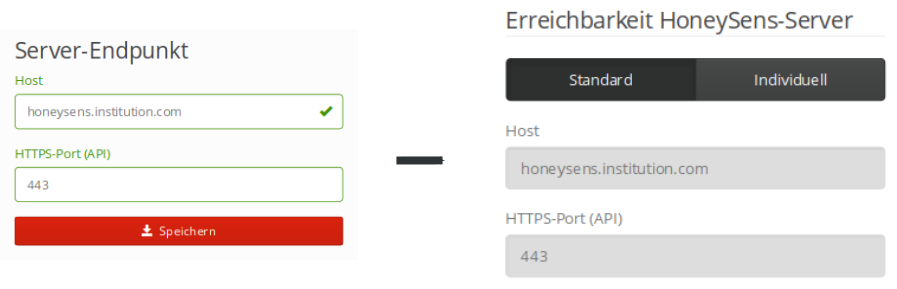
\includegraphics[width=\textwidth]{./graphics/endpoint-cert.png}
				\caption{Definition des Server-Endpunktes unter Nutzung eines gültigen Zertifikats}
				\label{fig:endpoint-cert}
\end{figure}

Abbildung \ref{fig:endpoint-cert} veranschaulicht diesen Umstand: Wenn der Common Name des für den Server genutzten TLS-Zertifikats von den Sensoren per DNS auflösbar ist, können beim Hinzufügen von Sensoren die systemweiten Standardwerte übernommen werden. Im Beispiel besitzt der Server ein gültiges TLS-Zertifikat für die Domain \verb|honeysens.institution.com|, die auch von den Sensoren entsprechend via DNS aufgelöst werden kann. Auch wenn dieser systemweite Wert jemals geändert werden sollte, aktualisieren die Sensoren diesen Wert automatisch. Dieses Setup stellt zugleich den vorgesehenen Einsatzzweck von HoneySens dar. Falls hingegen keine gesonderten Zertifikate für die Domain des HoneySens-Servers bei der Installation zur Verfügung gestellt werden, kommt automatisch ein selbstsigniertes Zertifikat zum Einsatz, das für jede Installation neu erzeugt wird. In diesem Fall ist es erforderlich, als globalen Endpunkten den im automatisch erzeugten Zertifikat hinterlegten Common Name als Endpunkt einzutragen, damit die Sensoren mit dem Server kommunizieren können. Da dieser vom System zufällig vergebene Common Name kein von den Sensoren auflösbarer Domainname ist, muss zufällig für jeden Sensor noch separat die IP-Adresse, unter der er den HOneySens-Server erreichen kann, spezifiziert werden. Diesen Umstand veranschaulicht beispielhaft Abbildung \ref{fig:endpoint-selfsigned}.

\begin{figure}[h]
				\centering
				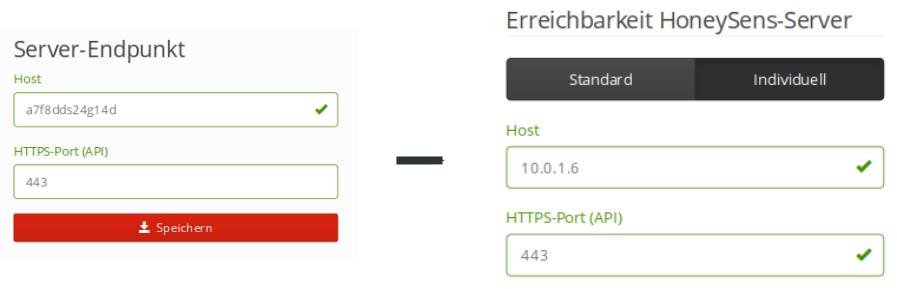
\includegraphics[width=\textwidth]{./graphics/endpoint-selfsigned.png}
				\caption{Definition des Server-Endpunktes mit selbstsigniertem Zertifikat}
				\label{fig:endpoint-selfsigned}
\end{figure}

Hier ist \verb|a7f8dds24g14d| der vom Server automatisch erzeugte Common Name des Zertifikates (typischerweise die ID der Docker-Instanz) und \verb|10.0.1.6| die IP-Adresse, aus der ein Sensor den Server erreichen kann.

\paragraph{SMTP-Konfiguration}
HoneySens kann automatisiert E-Mails versenden: Entweder, um Nutzer über kritische Vorfälle zu informieren oder zur Bereitstellung von wöchentlichen Zusammenfassungen über alle binnen der letzten sieben Tage aufgetretenen Ereignisse. Die Konfiguration, wann und an wen welche E-Mails verschickt werden sollen, ist Teil der Benutzerverwaltung und wird in Kapitel \ref{groups} beschrieben. Als Voraussetzung, damit dieser Mechanismus genutzt werden kann, ist allerdings zunächst noch die Konfiguration eines SMTP-Server notwendig, über den Mails an ihre Adressaten verschickt werden können. Das vorliegende Formular bietet hierfür die folgenden Felder an:

\begin{description}
				\item[Server]: Der via DNS auflösbare Hostname oder die IP-Adresse des zu nutzenden E-Mail-Servers.
				\item[Absender]: Die E-Mail-Adresse, die als Absender bei vom System generierten Nachrichten eingetragen werden soll.
				\item[Benutzer und Passwort]: \textit{optional}, wenn der Server Authentifizierung erfordert.
\end{description}

\newpage
\part{HowTos}
Dieser Abschnitt stellt exemplarisch vor, wie einige häufig durchzuführende Arbeitsschritte mit dem System durchgeführt werden können. Jedes Kapitel stellt einen solchen Workflow vor, indem zunächst das zu erreichende Ziel, die dafür notwendigen Voraussetzungen und anschließend die einzeln durchzuführenden Schritte erklärt werden.

\section{Einrichten eines neuen Sensors}
\paragraph{Ziel}
Es soll ein neuer Sensor vom Typ \textit{BeagleBone Black} zu einer Gruppe hinzugefügt und ans Netz gebracht werden.
\paragraph{Voraussetungen}
\begin{itemize}
				\item Nutzer ist mit einem Manager- oder Administratoraccount angemeldet (Kapitel \ref{login})
				\item Nutzer gehört der Gruppe an, in die der neue Sensor eingefügt werden soll (Kapitel \ref{groups})
				\item Gültige Firmware ist auf dem Server als Standardfirmware registriert (Kapitel \ref{firmware})
				\item Der globale Server-Endpunkt ist korrekt definiert (Kapitel \ref{system-settings})
				\item \textbf{Hardware}: BeagleBone Black, microSD-Karte (mind. 4GB), Kabel zur Netzwerk- und Stromversorgung
\end{itemize}
\paragraph{Vorgehensweise}
Zunächst muss der neue Sensor auf dem Server mit Hilfe der Webanwendung registriert werden. Hierfür wird zuerst das Modul \textit{Sensoren} in der Sidebar ausgewählt (1) und über der erscheinenden Liste der Button \textit{Hinzufügen} angeklickt (2).

\begin{figure}[h]
				\centering
				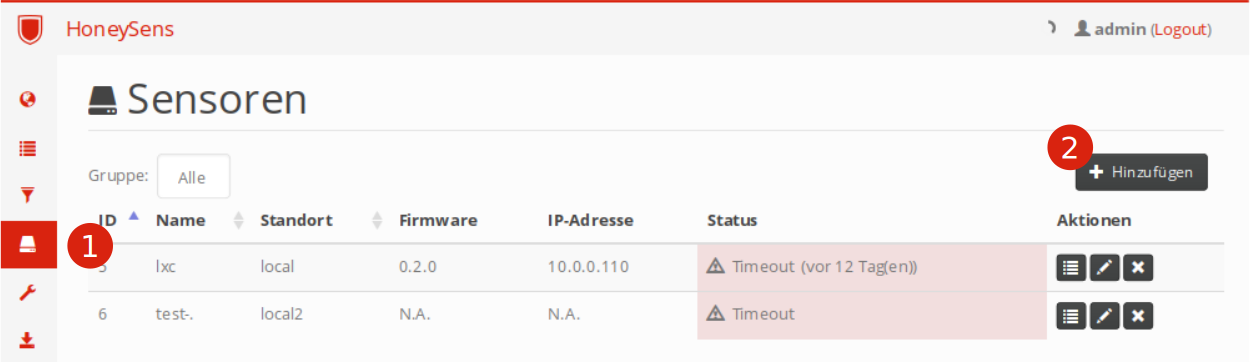
\includegraphics[width=\textwidth]{./graphics/howto-sensor-add-1.png}
				\label{fig:howto-sensor-add-1}
\end{figure}

Es erscheint ein Formular, in dem alle für den neuen Sensor relevanten Einstellungen vorgenommen werden. Zunächst gilt es, einen Namen für den Sensor zu vergeben (1). Dieser dient lediglich dazu, das Gerät über die Webanwendung und in der Ereignisliste leichter identifizieren zu können. Ebenso verhält es sich mit der Angabe des Standortes (2). Hier kann ein beliebiger String eingetragen werden, der das Auffinden des Geräts vor Ort erleichtern soll - beispielsweise eine Gebäude- oder Raumnummer. Außerdem muss mit einer Dropdown-Liste noch spezifiziert werden, welcher Gruppe das Gerät angeschlossen werden soll (3).

\begin{figure}[h]
				\centering
				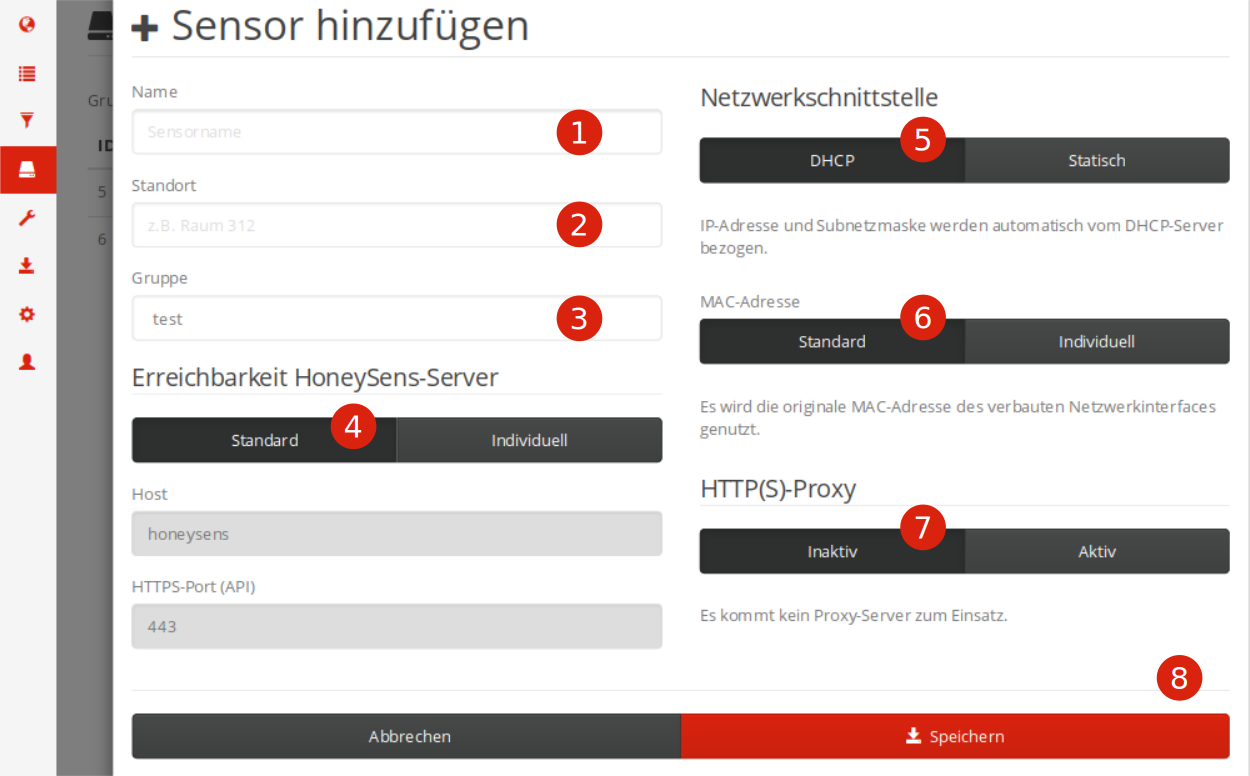
\includegraphics[width=\textwidth]{./graphics/howto-sensor-add-2.png}
				\label{fig:howto-sensor-add-2}
\end{figure}

Nach diesen allgemeinen Angaben können bei Bedarf noch weitere Einstellungen unter den Punkten \textit{„Erreichbarkeit HoneySens-Server“}, \textit{„Netzwerkschnittstelle“} und \textit{„HTTP(S)-Proxy“} vorgenommen werden. 

Falls der HoneySens-Server mit den unter \textit{Host} und \textit{HTTPS-Port} angegebenen globalen Daten vom neuen Sensor nicht erreichbar sein wird (weil beispielsweise im Zielnetz kein DNS-Server zur Auflösung des Hostnamens zur Verfügung steht), kann mit einem Klick auf \textit{Individuell} alternativ eine IP-Adresse angegeben werden (4). Wenn im Zielnetz kein DHCP-Server zur Verfügnung steht, kann unter \textit{Netzwerkschnittselle} mit einem Klick auf \textit{Statisch} auch eine individuelle IP-Adresse mit zugehöriger Netzmaske, Gateway und DNS-Server spezifziert werden. Außerdem kann bei Bedarf eine individuelle MAC-Adresse festgelegt werden (6). Standardmäßig kommt die originale Hardware-MAC-Adresse des Sensors unverändert zum Einsatz. Zuletzt ist es außerdem noch möglich, bei Bedarf HTTP(S)-Proxy-Server zu definieren. Dies ist nur nötig, wenn der HoneySens-Server nicht über normale Routen erreichbar ist und der einzige Weg zwingend über Proxy-Server führt. Nach einem Klick auf \textit{Aktiv} erscheint ein Formular, in dem die Adresse des zu verwendenden Proxy-Sservers und bei Bedarf auch Nutzername und Passwort festgelegt werden können (7). Die Sensorsoftware wird automatisch versuchen, das korrekte Authentifizierungsverfahren zu finden.

Wenn alle Einstellungen korrekt vorgenommen wurden, kann mit einem Klick auf \textit{Speichern} fortgefahren werden (8).

\begin{figure}[h]
				\centering
				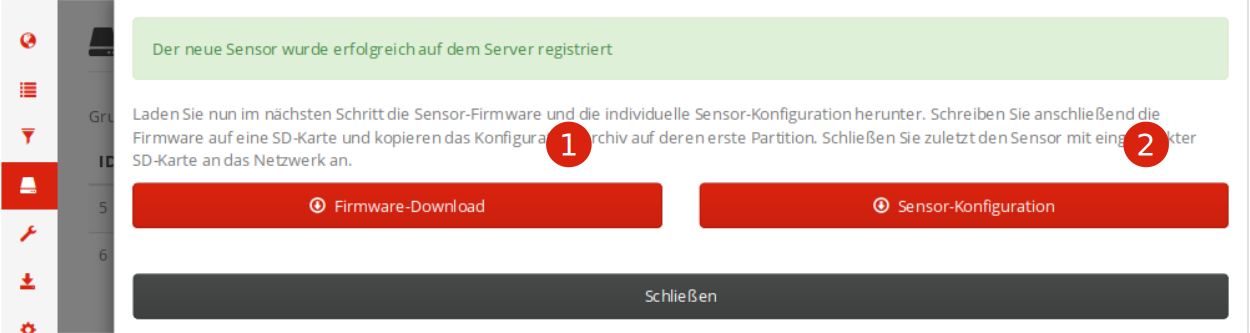
\includegraphics[width=\textwidth]{./graphics/howto-sensor-add-3.png}
				\label{fig:howto-sensor-add-3}
\end{figure}

Im anschließend erscheinenden Dialog werden zwei Dateien zum Download angeboten: Die generische Sensor-Firmware (1) und die an den Sensor angepasste Konfiguration (2). 

Das Firmware-Archiv beinhaltet ein Abbild eines Installers, das auf ein Installationsmedium (microSD-Karte) geschrieben werden muss und für alle Sensoren identisch ist. Dieses Archiv kann alternativ auch schon vor dem Einrichten eines Sensors im Modul \textit{Firmware} geosndert heruntergeladen werden. Damit ein Sensor aber nach der Installation mit seinen zuvor eingegebenen Konfigurationsdaten (Netzwerkkonfiguration, Erreichbarkeit Server usw.) versorgt werden kann, ist es vor der Installation noch notwendig, die Sensor-Konfiguration (2) auf das Installationsmedium zu kopieren.

Hinter dem Firmware-Download verbirgt sich ein Archiv mit der Endung \verb|.tar.gz|, das von den meisten Archivierungsprogrammen entpackt werden kann. Es beinhaltet zwei Dateien: den Installer selbst (\verb|firmware.img|) und eine Datei mit beschreibenden zugehörigen Metadaten (\verb|metadata.xml|), die für die Installation ignoriert werden kan(\verb|firmware.img|) und eine Datei mit beschreibenden zugehörigen Metadaten (\verb|metadata.xml|), die bei der Installation ignoriert werden kann. Zunächst gilt es, den Installer auf eine microSD-Karte zu schreiben. Unter unixoiden Betriebssystemen wie \textit{Linux} oder \textit{OSX} kann dies mit Hilfe des Tools \verb|dd| erfolgen. Unter \textit{Windows} kann beispielsweise \textit{WinDiskImager} genutzt werden. Nachfolgend exemplarisch das Auspacken und Schreiben der Firmware auf die microSD-Karte \verb|/dev/mmcblk0| unter Linux:
\begin{lstlisting}
$ tar xzf s1.tar.gz
$ ls
. .. firmware.img metadata.xml s1.tar.gz
$ dd if=./firmware.img of=/dev/mmcblk0 bs=4M
\end{lstlisting}
Sobald das Abbild erfolgreich auf das Installationsmedium geschrieben wurde, befindet sich darauf neben dem eigentlichen Installer auch eine 100 Megabyte große FAT-Partition, die zur Konfiguration genutzt wird unter beispielsweise unter Windows automatisch eingehangen wird. Auf diese Partition muss zuletzt noch das Konfigurationsarchiv (2) kopiert werden. \textbf{Hinweis:} Das Archiv mit den Konfigurationsdaten darf zuvor \textbf{nicht} entpackt werden! Dies kann unter unixoiden Systemen beispielsweise folgendermaßen aussehen:
\begin{lstlisting}
$ mount /dev/mmcblk0p1 /mnt
$ cp s1.tar.gz /mnt
$ umount /dev/mmcblk0p1
\end{lstlisting}
\begin{wrapfigure}{r}{0.5\textwidth}
				\vspace{-15pt}
				\centering
				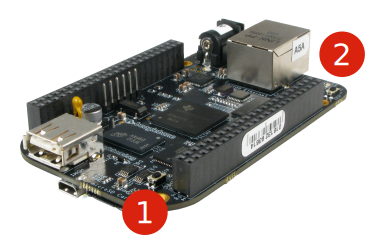
\includegraphics[width=0.48\textwidth]{./graphics/howto-sensor-add-4.png}
				\vspace{-5pt}
				\label{fig:howto-sensor-add-4}
\end{wrapfigure}

Die Vorbereitungen für die microSD-Karte als Installationsmedium sind an dieser Stelle abgeschlossen. Zuletzt gilt es, das Installationsmedium in den nebenstehend abgebildeten Sensor einzulegen, der Slot für die microSD-Karte befindet sich an Position (1). Das Gerät wird nach dem Einschalten von diesem Medium booten und die automatische Installation anstoßen, während der die Sensor-Firmware auf den internen Speicher des BeagleBone geschrieben wird. Im Anschluss erfolgt ein automatischer Neustart und das Gerät ist einsatzbereit. Zuvor ist noch zu berücksichtigen, dass die Stromversorgung und Netzwerkverbindung angeschlossen sind. Die entsprechenden Anschlüsse befinden sich an Position (2). Mit dem Einstecken der Stromversorgung wird der Sensor automatisch starten, die Installation durchführen und sich anschließend beim Server registrieren.

Die Installation eiens Sensors dauert je nach Geschwindigkeit des verwendeten Installationsmediums etwa 20 bis 30 Minuten. Um dies zu veranschaulichen, zeigen die vier blauen LEDs an Seite (2) während des Sensors während dieses Vorgangs ein Lauflicht an. Abschließend versucht der Sensor, den Server zu kontaktieren. Wenn dieser Kontakt erfolgreich war, wechselt der Status des Sensors in der Sensorübersicht auf \textit{online}. Der Sensor ist anschließend einsatzbereit und meldet verdächtige Ereignisse an den Server.

\begin{figure}[h]
				\centering
				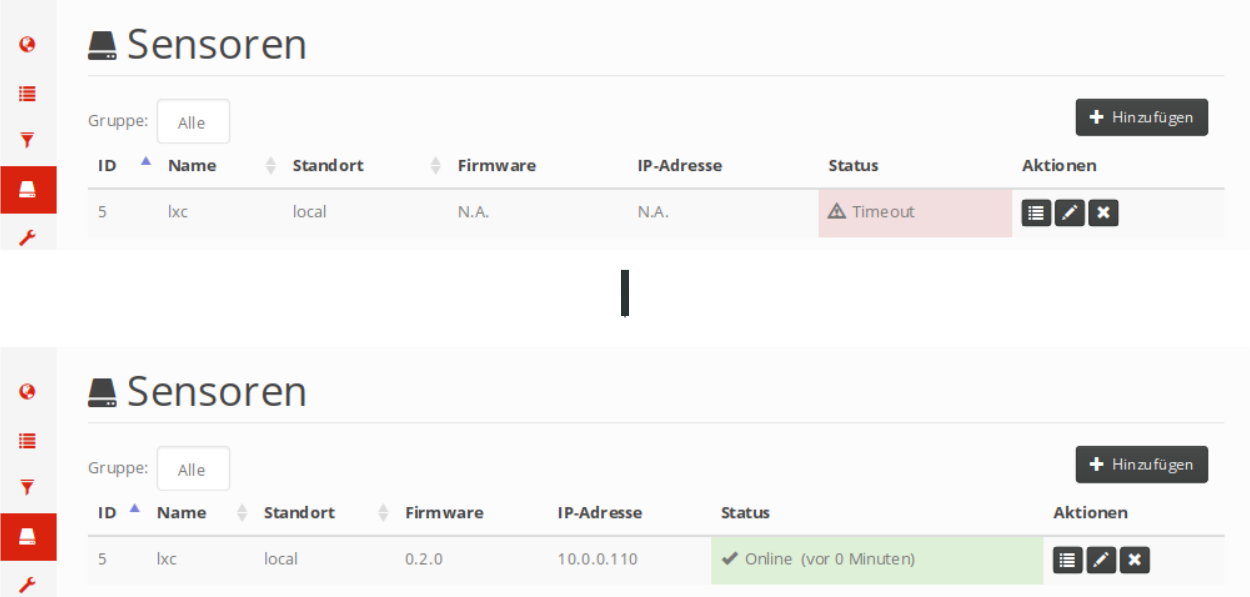
\includegraphics[width=\textwidth]{./graphics/howto-sensor-add-5.png}
				\label{fig:howto-sensor-add-5}
\end{figure}

\newpage
\section{Ereignisfilter anlegen}
\paragraph{Ziel}
Für wiederkehrende, als harmlos einzustufende Ereignisse einer bestimmten Quell-IP-Adresse soll ein Filter eingerichtet werden, damit zukünftige Vorfälle dieser Art nicht mehr gesondert aufgezeichnet werden (sog. \textit{Whitelisting}).
\paragraph{Voraussetungen}
\begin{itemize}
				\item Nutzer ist mit einem Manager- oder Administratoraccount angemeldet (Kapitel \ref{login})
				\item Nutzer gehört der Gruppe an, für die die neue Filterregel angelegt werden soll (Kapitel \ref{groups})
\end{itemize}
\paragraph{Vorgehensweise}
Zunächst gilt es, die Ereignisliste auszuwerten und alle nötigen Informationen zum Anlegen des Filters zu sammeln. Dazu wird das Modul \textit{Ereignisse} über die Sidebar aufgerufen und die Sicht auf die Liste, falls nötig, mit Hilfe der Filterfunktionen im oberen Bereich angepasst (siehe auch Kapitel \ref{eventlist}).
\begin{figure}[h]
				\centering
				\includegraphics[width=\textwidth]{./graphics/howto-event-filter-1.png}
				\label{fig:howto-event-filter-1}
\end{figure}
Im Beispiel ist zu sehen, dass wiederholt eine Reihe von Ereignissen von der IP-Adresse 10.0.0.1 verursacht wurden. Mit Klick auf den Button \textit{Details} (1) werden zusätzliche Informationen zu einem gewählten Ereignis sichtbar. In diesen Details kann mit einem Klick auf \textit{Paketübersicht} eine Liste aller vom entfernten Host (und somit potentiellen Angreifer) empfangenen Datenpakete eingesehen werden, die zu diesem Ereignis zugeordnet wurden.
\begin{figure}[h]
				\centering
				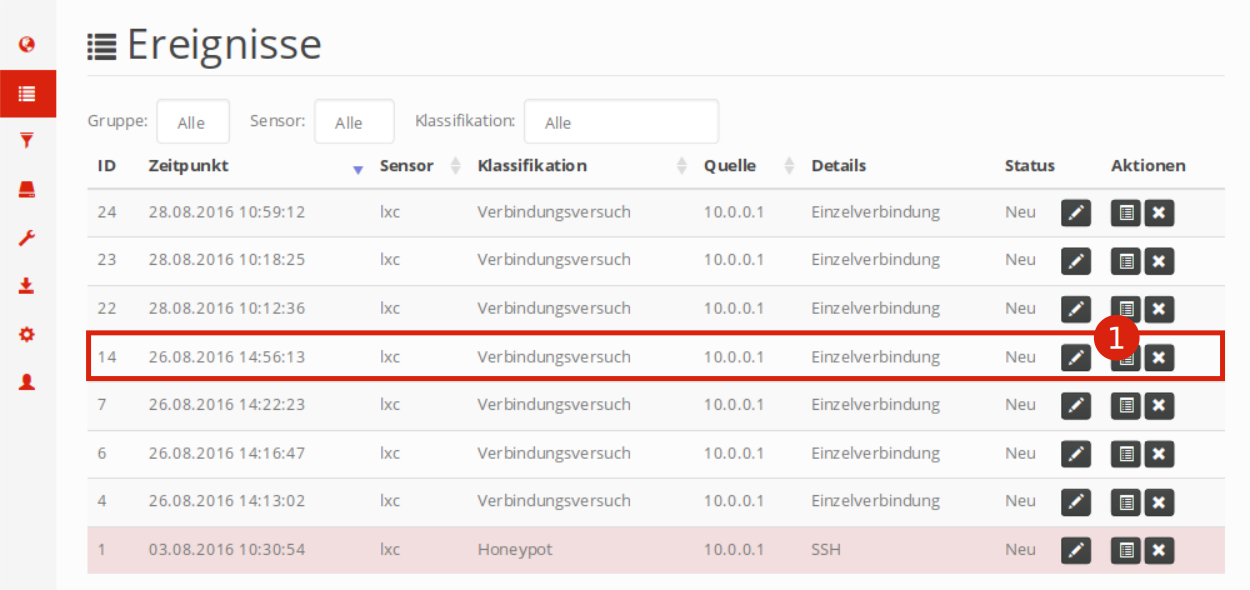
\includegraphics[width=\textwidth]{./graphics/howto-event-filter-2.png}
				\label{fig:howto-event-filter-2}
\end{figure}
Beispielhaft erfahren wir, dass der Sensor mit dem Namen \verb|lxc| das Ereignis aufgezeichnet hat und alle Pakete an den TCP-Port 312 gerichtet waren. Durch Nachforschungen im Produktivnetz finden wir beispielsweise heraus, dass es sich bei dem Rechner mit der IP-Adresse 10.0.0.1 um ein anderes der IT-Sicherheit dienliches System handelt, das mit derartigen Anfragen das Netzwerk scannt, um Hosts zu finden, die Online sind. Nun gilt es, eine Filterregel hinzuzufügen, um solche Vorgänge zukünftig nicht mehr als Vorfall zu melden.

Im ersten Schritt wird das Modul für die Ereignisfilter mit einem Klick auf \textit{Filter} in der Sidebar gestartet (1).
\begin{figure}[h]
				\centering
				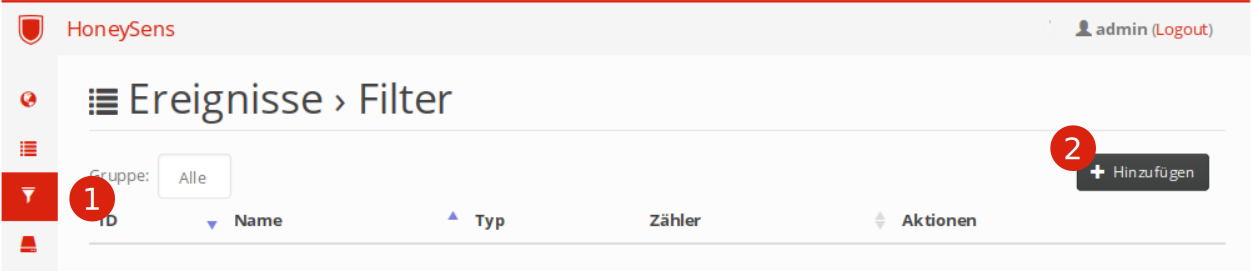
\includegraphics[width=\textwidth]{./graphics/howto-event-filter-3.png}
				\label{fig:howto-event-filter-3}
\end{figure}
Es wird eine Liste aller Filter dargestellt, die für die gewählte Gruppe (bzw. standardmäßig alle Gruppen, denen der aktuelle Benutzer angehört) registriert wurden. Ein Klick auf den Button \textit{Hinzufügen} ruft den Dialog zum Speichern neuer Filter auf, der nachfolgend dargestellt ist (2).

\newpage
\begin{figure}[h]
				\centering
				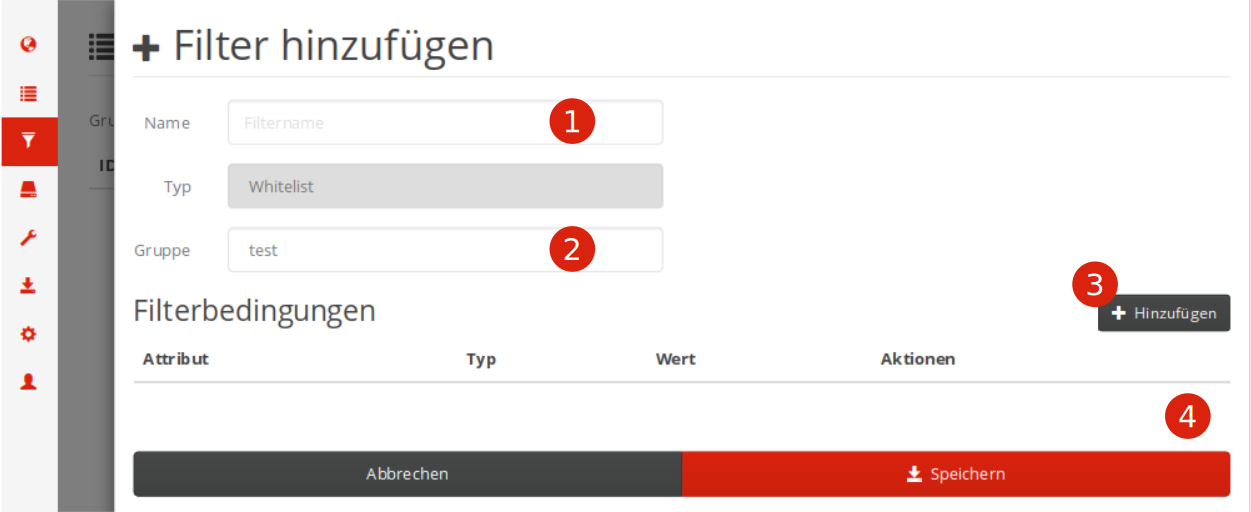
\includegraphics[width=\textwidth]{./graphics/howto-event-filter-4.png}
				\label{fig:howto-event-filter-4}
\end{figure}

Grundsätzlich muss für jeden Filter zunächst ein beliebiger Name (1) vergeben werden, der den Filter innerhalb der Webanwendung identifiziert. Weiterhin ist jeder Filter einer fixen Gruppe zugewiesen (2) und auch nur für die Sensoren und Ereignisse innerhalb dieser Gruppe gültig. Da IP-Adressen in verschiedenen Teilnetzen durchaus mehrmals vergeben sein können, sind global gültige Filterregeln problematisch und werden deshalb nicht unterstützt.

Herzstück des Filtersystems sind die Filterregeln. Jeder Filter setzt sich aus einer Reihe von Regeln zusammen und wird erst auf ein Ereignis angewandt, wenn \textbf{ALLE} dieser Regeln zutreffen. Es handelt sich folglich um eine logische UND-Verknüpfung der einzelnen Regeln. Um neue Regeln hinzuzufügen, wird der gleichnamige Button genutzt (3). Anschließend erscheint in der Liste der Filterbedingungen eine neue einzeilige Regel.

\begin{figure}[h]
				\centering
				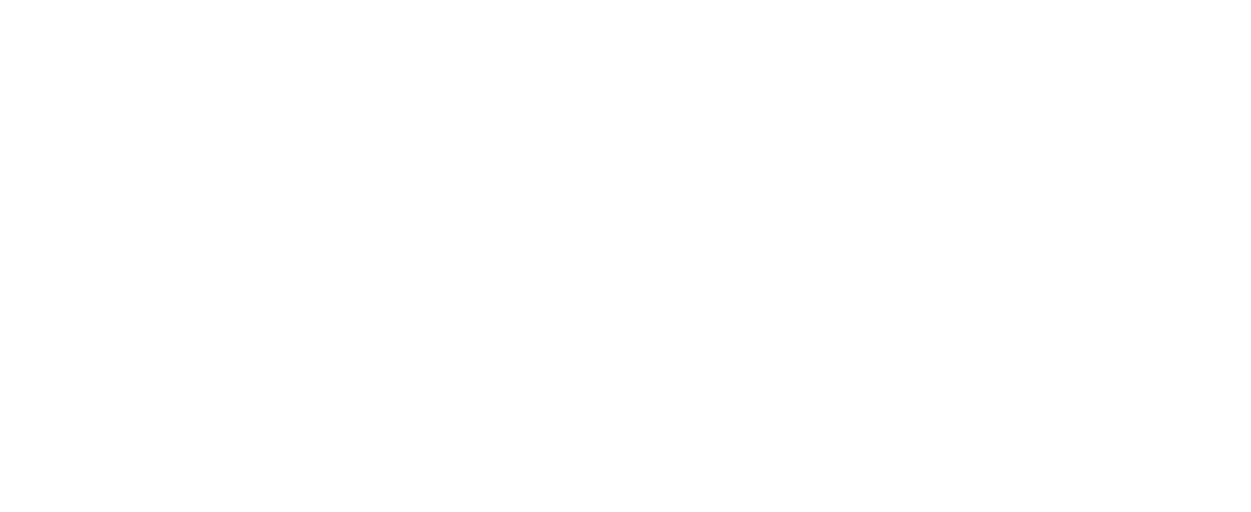
\includegraphics[width=\textwidth]{./graphics/howto-event-filter-5.png}
				\label{fig:howto-event-filter-5}
\end{figure}

Jede individuelle Regel besteht aus einem Attribut (A), einer \textit{Typ} genannten genaueren Spezifizierung (B, je nach Attribut) und einer Wertzuweisung (C). Wenn das gewählte Attribut in den angegebenen Wertebereich fällt, gilt die Regel als erfüllt. Die obige Abbildung gibt alle drei Regeln an, die unseren Beispiel-Filter umfassen:
Pakete von
\begin{itemize}
				\item der Quell-IP-Adresse 10.0.0.1 (das Sicherheitssystem),
				\item die das TCP-Protokoll nutzen und
				\item auf dem Zielport 312 eintreffen
\end{itemize}
werden fortfan vom System auf die Whitelist gesetzt und ignoriert. Wenn alle Regeln ordnungsgemäß eingerichtet sind, kann der Filter mit einem Klick auf \textit{Speichern} auf dem Server registriert und aktiviert werden. Nach dem Anlegen des Filters wird wieder die Filterliste sichtbar, in der ein neuer Eintrag betrachtet werden kann. Der enthält neben dem Namen auch einen Zähler, der immer um eins erhöht wird, wenn ein Ereignis eintrifft, das den Filterbedingungen entspricht und somit verworfen wird. Mit Hilfe des Zählers kann die Wirksamkeit eines Filters leicht überprüft werden (A).

\begin{figure}[h]
				\centering
				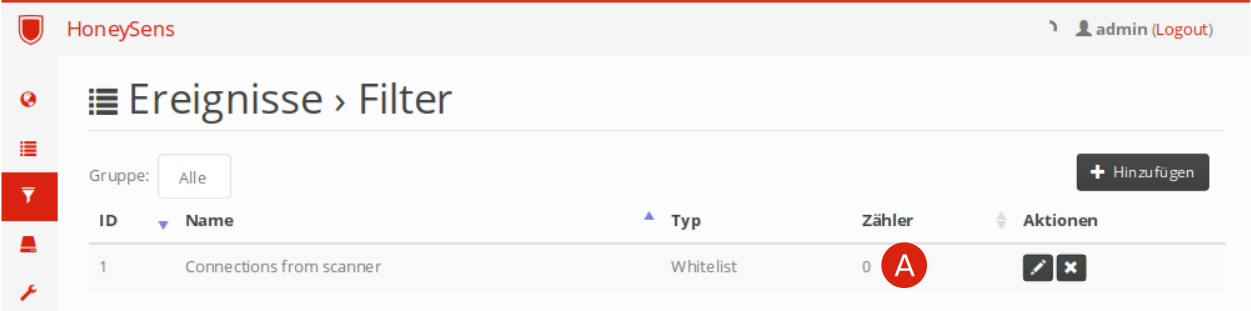
\includegraphics[width=\textwidth]{./graphics/howto-event-filter-6.png}
				\label{fig:howto-event-filter-6}
\end{figure}
\end{document}
